\chapter{مسیریابی}\label{ch path planning}

\section{مقدمه}

به طراحی مسیری امن به طوری که بدون برخورد با موانع از قرارگیری اولیه، که شامل مکان و زاویه‌ها، به طور کلی تمام پارامترهای توصیف یک جسم در فضای محیط، به قرارگیری نهایی است، مسیریابی\LTRfootnote{path planning} می‌گویند. در این پروژه می‌توان مکان ربات‌ها و موانع را به عنوان حالت\LTRfootnote{state} در نظر گرفت. با توجه به اینکه دید از بالا فرض شده است به نحوی که از تمام مکان‌ها اطلاع داشته باشیم، در نتیجه نسبت به تمام موانع اطلاع دقیقی داریم. پس می‌توان گفت در هر حالت نسبت به محیط و داده‌ها به طور کامل مطلع\LTRfootnote{informed} هستیم. در این فصل ابتدا روش میدان پتانسیل و سپس الگوریتم‌های مسیریابی مبتنی بر روش‌های ابتکاری\LTRfootnote{heuristic} که لازمه آن‌ها مطلع بودن از محیط است، پیاده‌سازی و بررسی گشته‌اند.

\section{میدان پتانسیل}
در این روش یک میدان دافعه و جاذبه ایجاد می‌کنیم و ربات در راستای میدان حرکت خواهد کرد. ایده اصلی این است که نقطه‌ی هدف را به صورت جاذبه و نقاطی که مانع هستند را به صورت دافعه در نظر بگیریم (همانند میدان الکتریکی و بارهای همنام و ناهمنام). در نتیجه، ربات به سمت نقطه هدف کشیده خواهد شد.

\subsection{روابط میدان پتانسیل}
رابطه میدان پتانسیل جذبی برای \lr{i}امین ربات از طرف بار ناهمنام یا به عبارتی موقعیت هدف که یک چاه پتانسیل سهمی‌گون ایجاد می‌کند، به شرح زیر است \cite{spong2006robot}:
\begin{equation}\label{eq Uatt}
U_{att,i} = 
\begin{cases*}
\frac{1}{2}\zeta_i\|o_i(q) - o_i(q_f)\|^2 & \lr{if} $\|o_i(q) - o_i(q_f)\| \le d$ \\
d\zeta_i\|o_i(q) - o_i(q_f)\|-\frac{1}{2}\zeta_id^2 & \lr{otherwise}
\end{cases*}
\end{equation}

که در آن منظور از $o_i(q_i)$ موقعیت ربات \lr{i}ام، $o_i(q_f)$ موقعیت مطلوب ربات، $\zeta_i$ ضریبی است که بعدا در روش گرادیان نزولی به ضریب آن تبدیل می‌گردد و $d$ فاصله گذر از چاه مخروطی را تعیین می‌کند. علت تعریف میدان به صورت فوض این است که در مرز $d$ هر دو برابر باشند و ناپیوستگی نداشته باشیم.

می‌دانیم $F_{att,i} = -\nabla U_{att,i}$ در نتیجه به توجه به رابطه \ref{eq Uatt} خواهیم داشت:
\begin{equation}
F_{att,i} = 
\begin{cases*}
-\zeta_i(o_i(q) - o_i(q_f)) & \lr{if} $\|o_i(q) - o_i(q_f)\| \le d$ \\
-d\zeta_i \frac{(o_i(q) - o_i(q_f))}{\|o_i(q) - o_i(q_f)\|} & \lr{otherwise}
\end{cases*}
\end{equation}

برای جلوگیری از برخورد با موانع میدان پتانسیل دفعی به صورت زیر تعریف کرد. این میدان ربات را از موانع دور کرده و اجازه برخورد ربات با مانع را نمی‌دهد. همچنین وقتی ربات از مانع دور است نباید نیرویی از طرف مانع به ربات اعمال گردد. به همین دلیل تابع پتانسیل باید طوری تعریف شود که به هنگام رسیدن ربات به مانع مقدارش بی‌نهایت و در یک فاصله مشخص از مرز مانع صفر گردد. این تابع پتانسیل برای ربات \lr{i} و مانع \lr{j}| به شکل زیر تعریف می‌گردد:
\begin{equation}\label{eq Urep}
U_{att,ij} = 
\begin{cases*}
\frac{1}{2}\eta_{ij}(\frac{1}{\rho_j(o_i(q))} - \frac{1}{\rho_{0j}})^2 & \lr{if} $\rho_j(o_i(q)) \le \rho_{0j}$\\
~~~~~~~~~~~0 & \lr{otherwise}
\end{cases*}
\end{equation}

که در آن $\rho_j(o_i(q))$ و $\rho_{0j}$ به ترتیب برابر یا کوتاه‌ترین فاصله بین $i$امین ربات و $j$امین مانع، و فاصله تاثیر $j$امین مانع هستند. با رابطه $F_{rep,ij} = -\nabla U_{rep,ij}$ و \ref{eq Urep} خواهیم داشت:
\begin{equation}\label{eq Frep}
F_{att,ij} = 
\begin{cases*}
\eta_{ij}(\frac{1}{\rho_j(o_i(q))} - \frac{1}{\rho_{0j}}) \frac{1}{\rho^2_j(o_i(q))} \frac{o_i(q)-o_j(q)}{\|o_i(q)-o_j(q)\|} & \lr{if} $\rho_j(o_i(q)) \le \rho_{0j}$\\
~~~~~~~~~~~0 & \lr{otherwise}
\end{cases*}
\end{equation}

در نهایت نیروی کل اعمالی به ربات به صورت زیر خواهد بود:
\begin{equation}\label{eq Ftot}
	F_{tot,i} = F_{att,i} + \sum_{j \in obstacles}^{}F_{rep,ij}
\end{equation}

در ادامه نحوه استفاده از نیرو توضیح داده خواهد شد.

\subsection{کنترل مسیر ربات با میدان پتانسیل}
برای این هدف نیروی اعمالی به ربات که در قسمت قبل محاسبه شد را به عنوان سرعت مطلوب به کنترل‌کننده تک ربات اعمال کردیم تا ربات به سرعت، مسیر خود را تغییر و به جهت مناسب حرکت نماید. مسیر پیموده شده توسط ربات با میدان پتانسیل در شکل \ref{Fig potential-field-1robot-pos} آمده است.
\begin{figure}[!h]
	\centering
	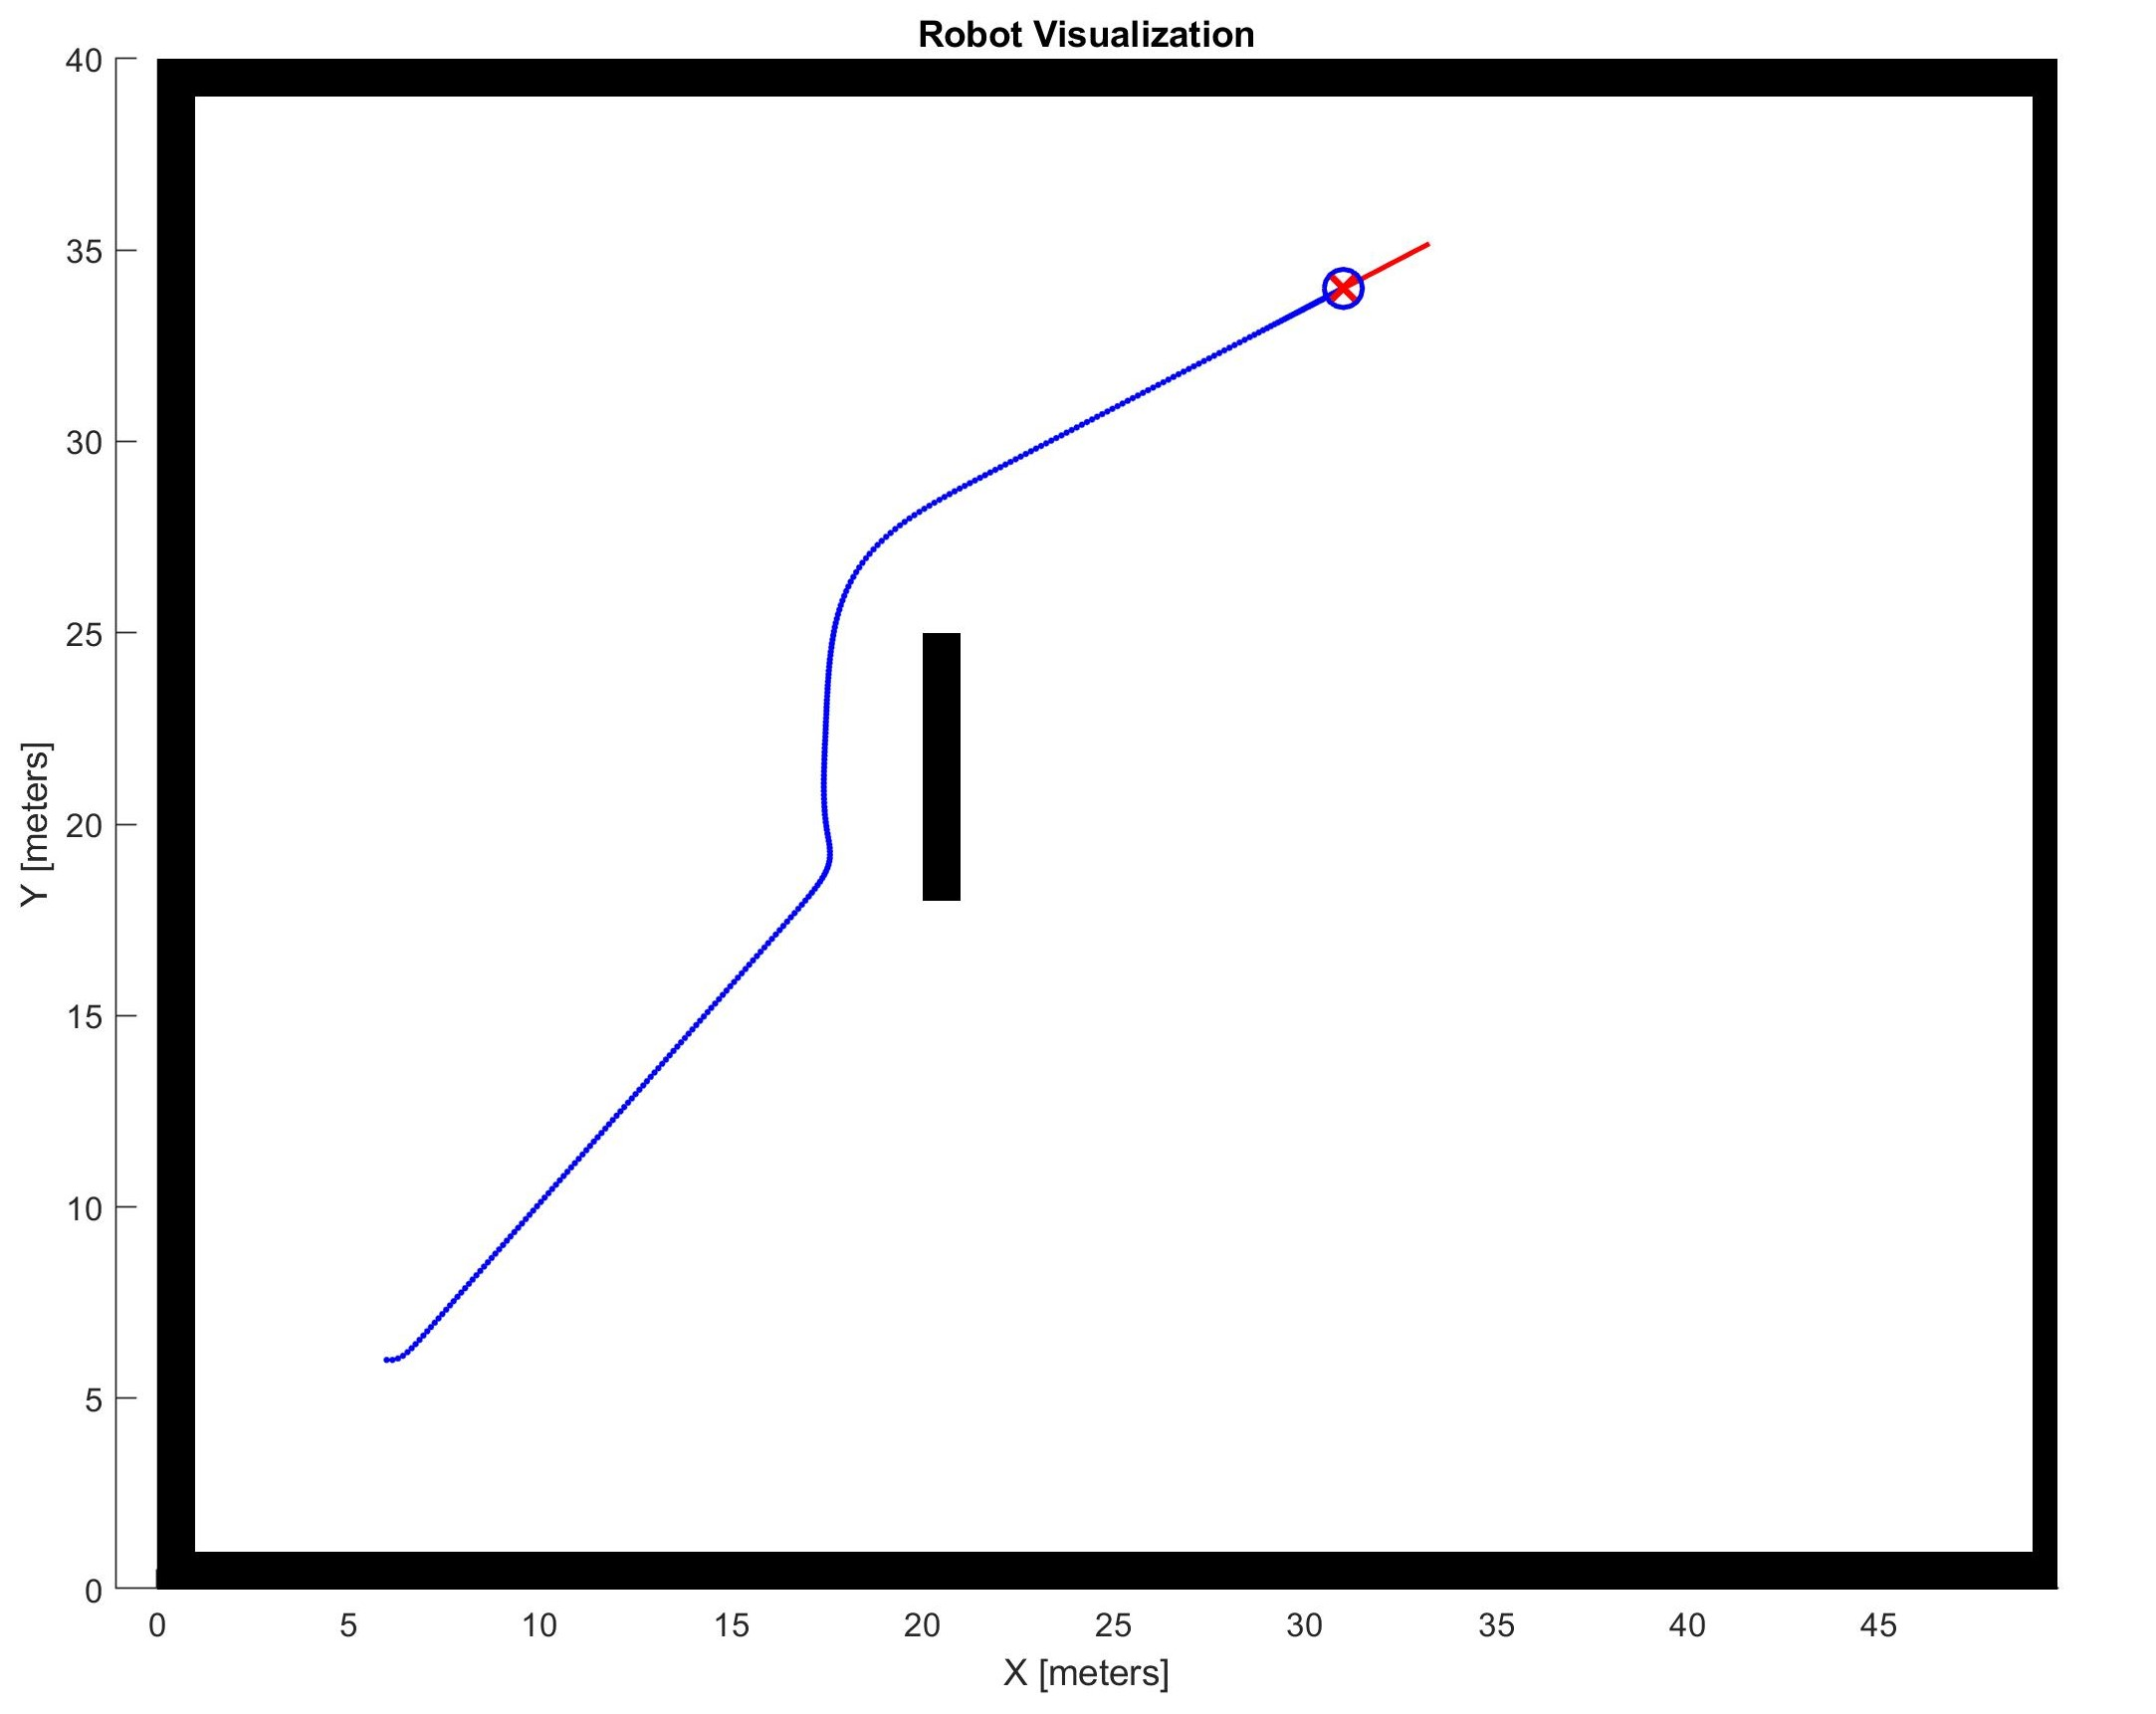
\includegraphics[scale=0.28]{Images/potential-field-1robot-pos.jpg}
	\caption{مسیر پیموده شده توسط ربات با میدان پتانسیل}\label{Fig potential-field-1robot-pos}
\end{figure}

یکی از مشکلات اصلی میدان پتانسیل این است که لزوما جواب ندارد و امکان دارد ربات در کمینه\LTRfootnote{minimum} محلی متوقف شود. به عنوان مثال در شکل \ref{Fig potential-field-1robot-stuck}، ربات در کمینه محلی گیر کرده و به نقطه هدف نرسیده است.
\begin{figure}[!h]
	\centering
	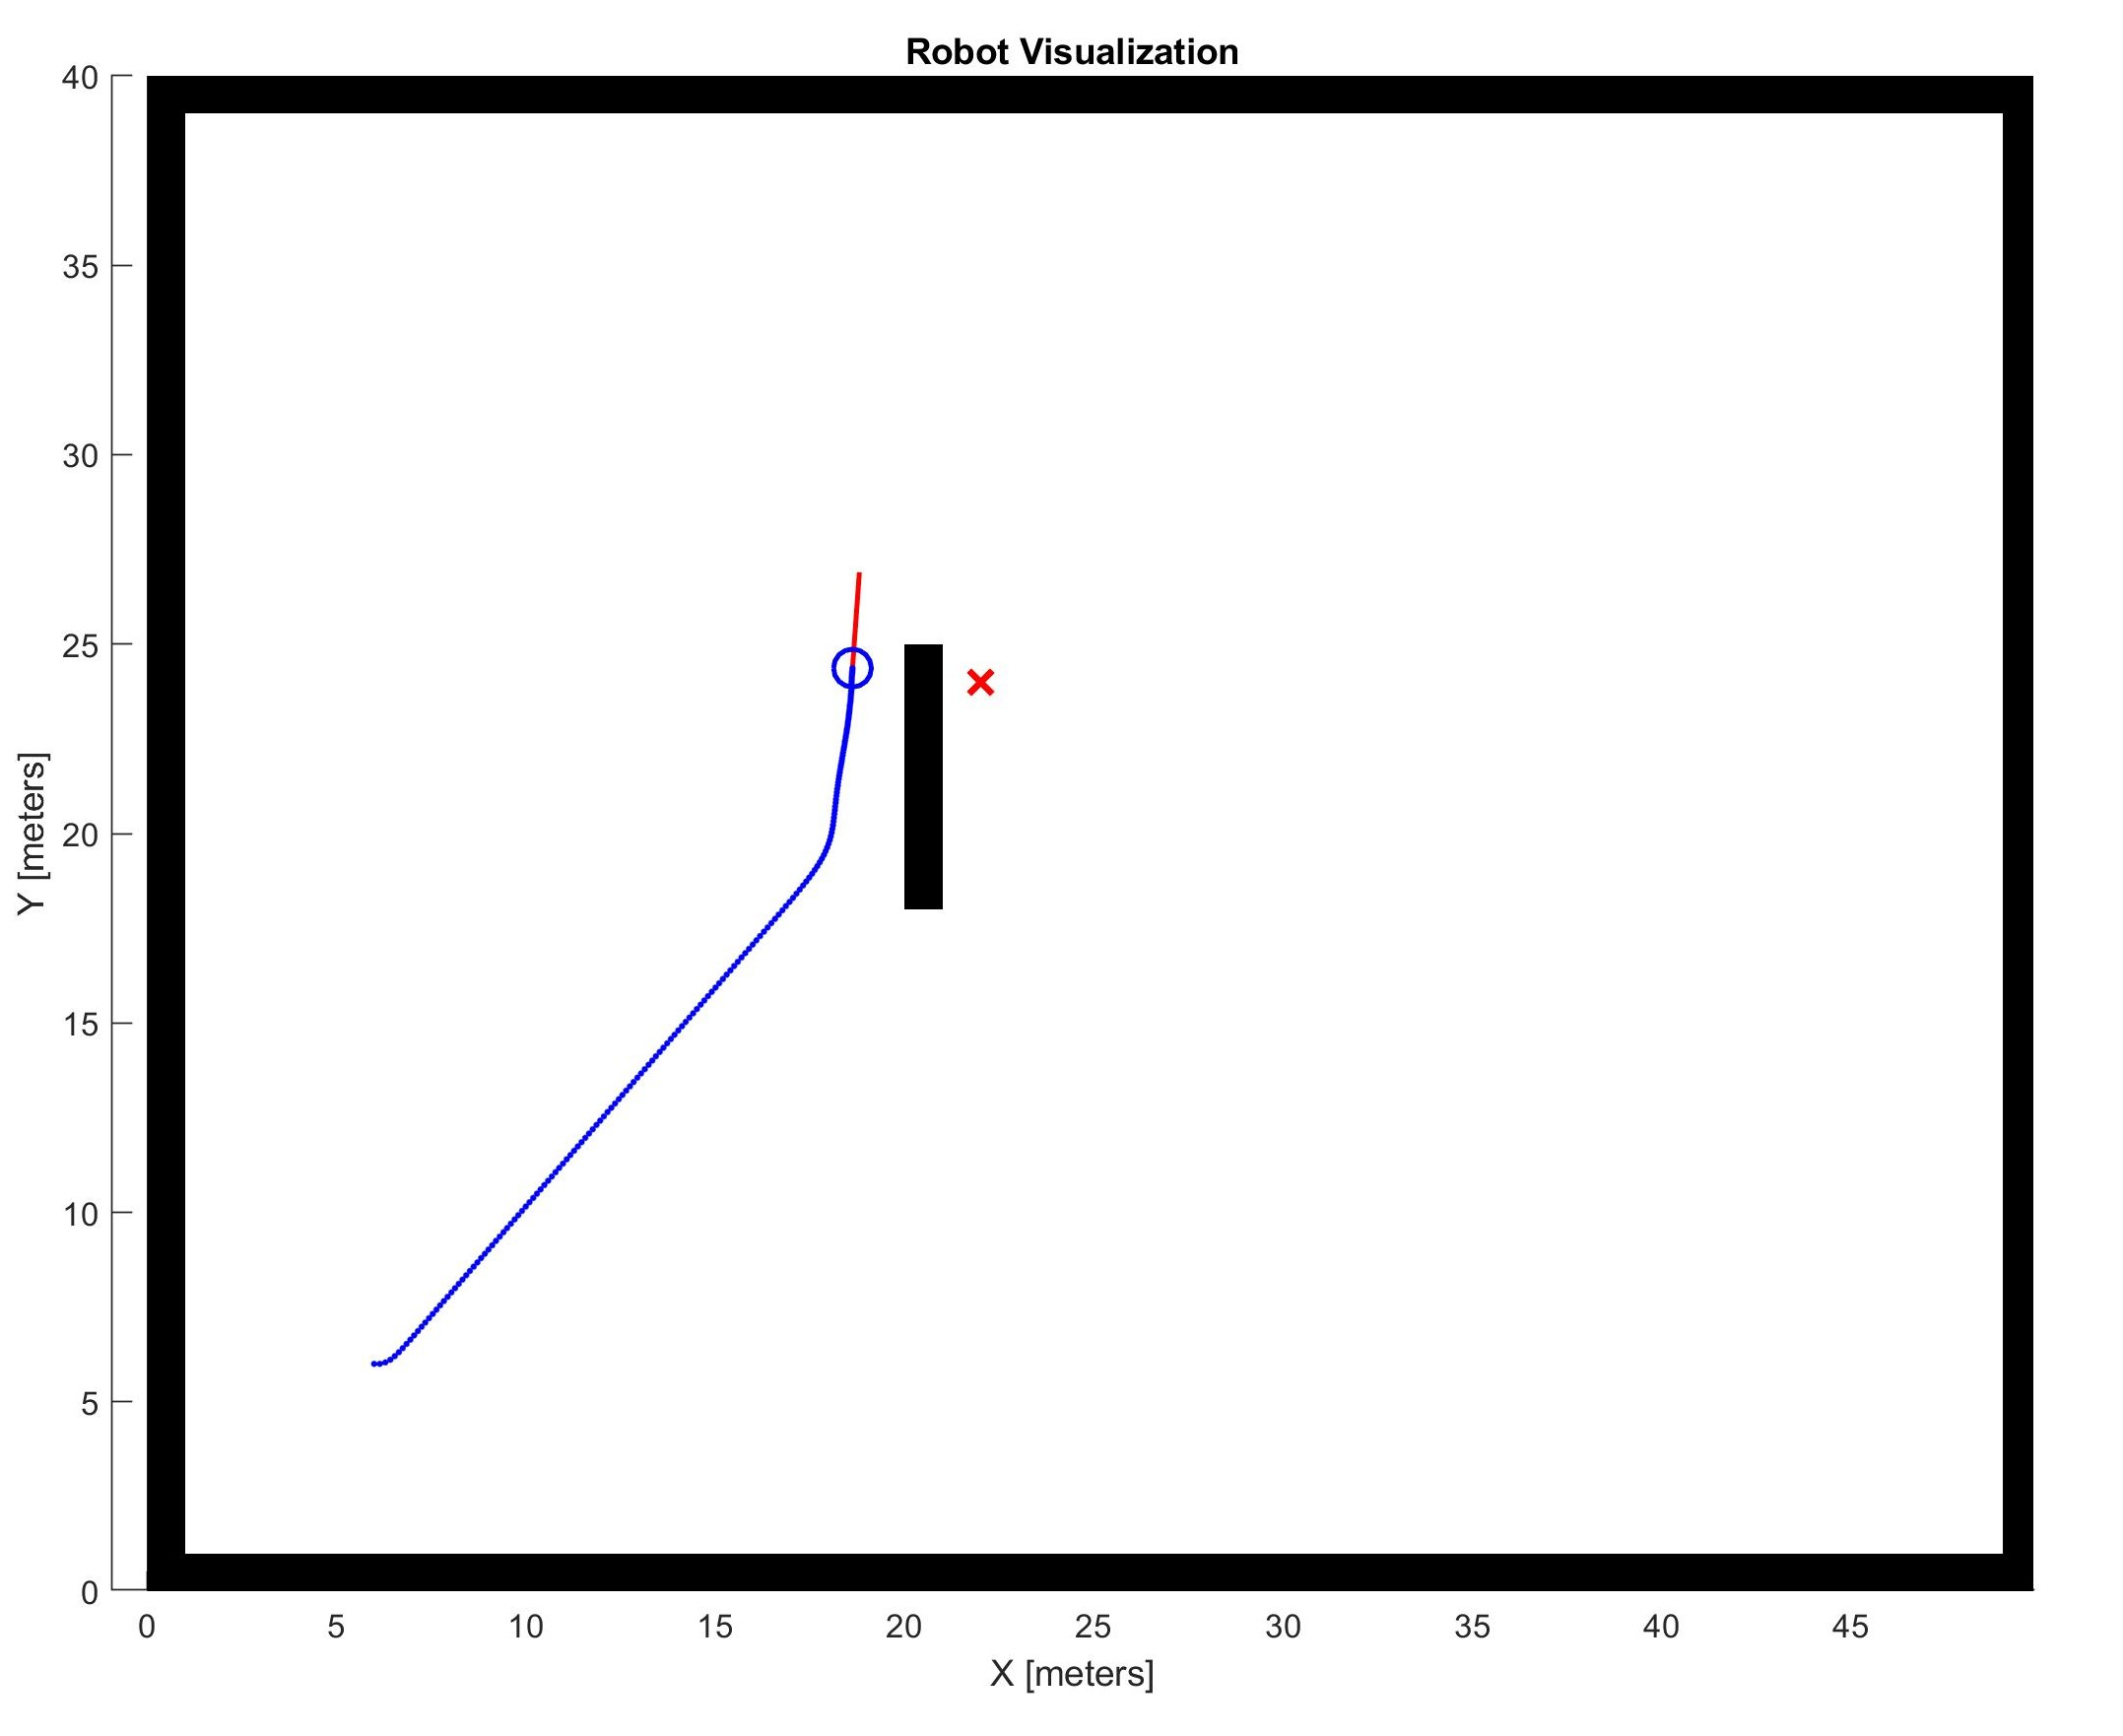
\includegraphics[scale=0.28]{Images/potential-field-1robot-stuck.jpg}
	\caption{گیر کردن ربات در کمینه محلی با میدان پتانسیل}\label{Fig potential-field-1robot-stuck}
\end{figure}

برای حل این مشکل معمولا نیرویی در جهت تصادفی به ربات وارد می‌گردد اما همچنان تضمینی برای خارج شدن از کمینه محلی\LTRfootnote{local minimum} وجود ندارد. لذا در ادامه به بررسی الگوریتم‌هایی می‌پردازیم که مطمئن هستیم حتما مسیری که به موقعیت مطلوب ختم می‌شود را می‌یابند.

\section{الگوریتم‌های ابتکاری}
همانطور که گفته شد، با توجه به شرایط مسئله و مطلع بودن در زمان طراحی مسیر، از الگوریتم‌های ابتکاری استفاده شده است. خصوصیت این الگوریتم‌ها در این است که با ابتکاری که به خرج داده می‌شود، مسئله اندکی ساده‌تر فرض شده و حل می‌گردد. مزیت این الگوریتم‌ها پیچیدگی زمانی کمتر آن‌ها نسبت به مسائلی هستند که مسئله مسیریابی را به طور کامل حل می‌نمایند. این امر در کاربرد رباتیک به دلیل اهمیت بلادرنگ\LTRfootnote{real time} بودن، دارای اهمیت بسیار زیادی می‌باشد. اما همانطور که گفته شد، چون مسئله به طور کامل حل نمی‌گردد، تضمینی برای رسیدن به پاسخ بهینه\LTRfootnote{optimal} وجود ندارد اما پاسخ به طور کلی معقول است، هر چند بهینه نباشد.

برای اعمال این الگوریتم‌ها نیاز به داشتن تعداد حالات محدود بود اما در بازه بین دو عدد متمایز در اعداد حقیقی، مجموعه حالات نامتناهی هستند. لذا از روش نمونه‌برداری\LTRfootnote{sampling based method} استفاده شد. در این پروژه، تمام نقاط با مختصات‌های اعداد صحیح را به عنوان حالت‌ها در نظر گرفتیم. همچنین مجموعه اقدامات\LTRfootnote{actions} به صورت حرکت به حالت‌های مجاور در راستاهای شمال، جنوب، شرق و غرب، و همچنین در راستاهای مورب شمال-غرب، شمال-شرق، جنوب-غرب و جنوب-شرق، تعریف شدند. مسیر خروجی نیز به صورت مجموعه‌ای مرتب از مختصات‌های مجاور که شروع آن مختصات اولیه و پایان آن مختصات نهایی می‌باشد، است. در این پروژه روش‌های ابتکاری \lr{BFS}\LTRfootnote{Breadth-first search}، \lr{Greedy best-first search} و $A^*$ پیاده سازی شده‌اند که در ادامه به توضیح آن‌ها می‌پردازیم.

\subsection{الگوریتم $BFS$}
الگوریتم \lr{BFS} در اصل یکی از الگوریتم‌های سرچ معروف و پایه‌ای گراف می‌باشد. برای استفاده از این روش، گراف را به نحوی که هر راس نماینده فقط و فقط یک حالت مجاز، و همچنین هر اقدام نماینده فقط و فقط یک یال باشد ساختیم. همچنین وزن هر یال برابر با نرم-2\LTRfootnote{2-norm} بردار جابه‌جایی اقدام مربوطه، که همان فاصله در مختصات دکارتی است، در نظر گرفته شد. منظور از حالت مجاز، مختصاتی است که در آن مانع نباشد و در محدوده کاری قرار گیرد. حال الگوریتم \lr{BFS} بر روی گراف اعمال می‌شود. قابل ذکر است در صورتی که وزن تمام یال‌ها برابر باشند، اثبات می‌گردد که این الگوریتم به جواب بهین خواهد رسید.

نحوه کار این الگوریتم به این صورت است که با شروع از راس شروع، راس‌های مجاور بررسی می‌شوند و سپس وارد یک صف\LTRfootnote{queue} می‌گردند تا راس‌های مجاور آن‌ها بررسی گردد. صف در ابتدا تنها دارای راس شروع است. برای اینکه راس‌های تکراری وارد صف نگردند، از رنگ‌آمیزی راسی استفاده شد. به این صورت که در ابتدا همه راس‌ها سفید و تنها راس شروع، مشکی می‌باشد. سپس هر راسی که وارد صف می‌شود به رنگ مشکی در می‌آید. در نتیجه هنگام بررسی راس‌های مجاور ابتدا بررسی می‌گردد که چه رنگی دارد. زیرا اگر مشکی باشد یعنی قبلا بررسی شده و دیگر نیازی به بررسی نیست. اینکار تا زمانی که به راس هدف برسیم، ادامه خواهد یافت.

اگر گراف به صورت 
$G = (V, E)$
که در آن \lr{V} مجموعه راس‌ها و \lr{E} مجموعه یال‌ها می‌باشد، تعریف شود، الگوریتم اصلی \lr{BFS} در شکل \ref{Fig BFS Algorithm} به صورت شبه کد آمده است \cite{cormen2009introduction}. منظور از نماد \lr{Q} در شبه کد، صف، منظور از \lr{d} فاصله و منظور از $\pi$ والد\LTRfootnote{parent} است. تفاوت در کد ارائه شده در این پروژه با این شبه کد، این است که احتیاجی به رنگ خاکستری نبود و رنگ خاکستری معادل رنگ مشکی در نظر گرفته شد. همچنین چون نقطه هدف داشتیم، در صورتی که به نقطه هدف می‌رسیدیم، حلقه خط 10 شکسته می‌شد و الگوریتم متوقف می‌گشت.
\begin{figure}[!h]
	\centering
	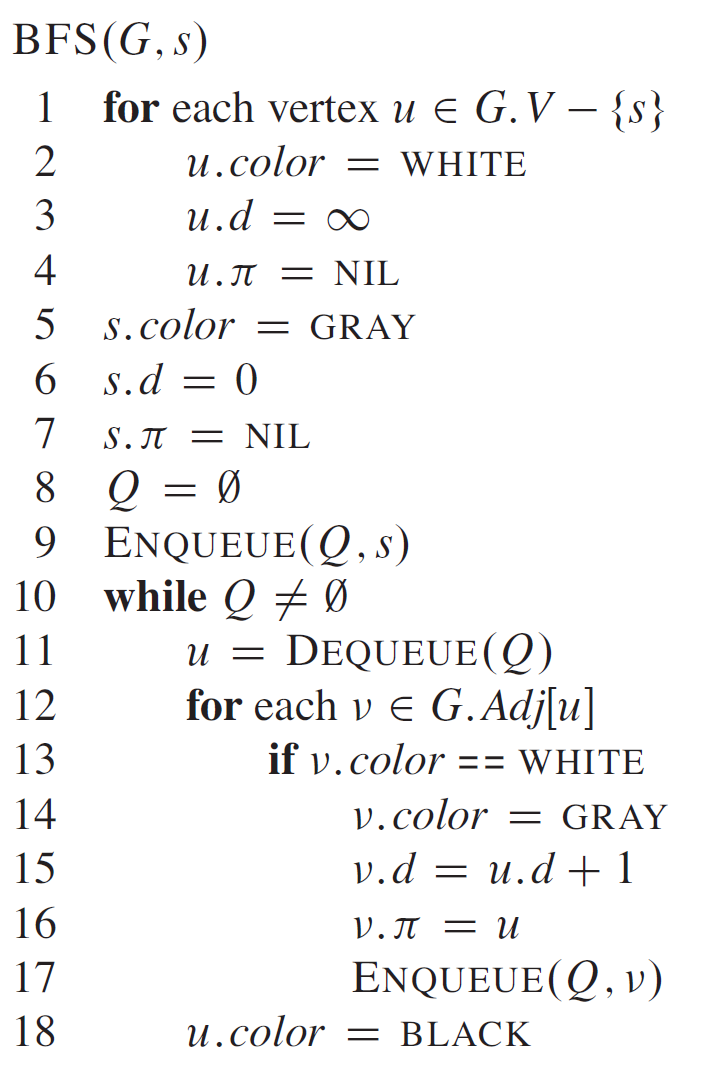
\includegraphics[scale=0.4]{Images/BFS-algorithm.png}
	\caption{شبه کد الگوریتم $BFS$}\label{Fig BFS Algorithm}
\end{figure}

 در شکل \ref{Fig BFS representation} نیز نحوه اعمال شدن الگوریتم \lr{BFS} بر روی یک گراف، نمایش داده شده است.
\begin{figure}[!h]
	\centering
	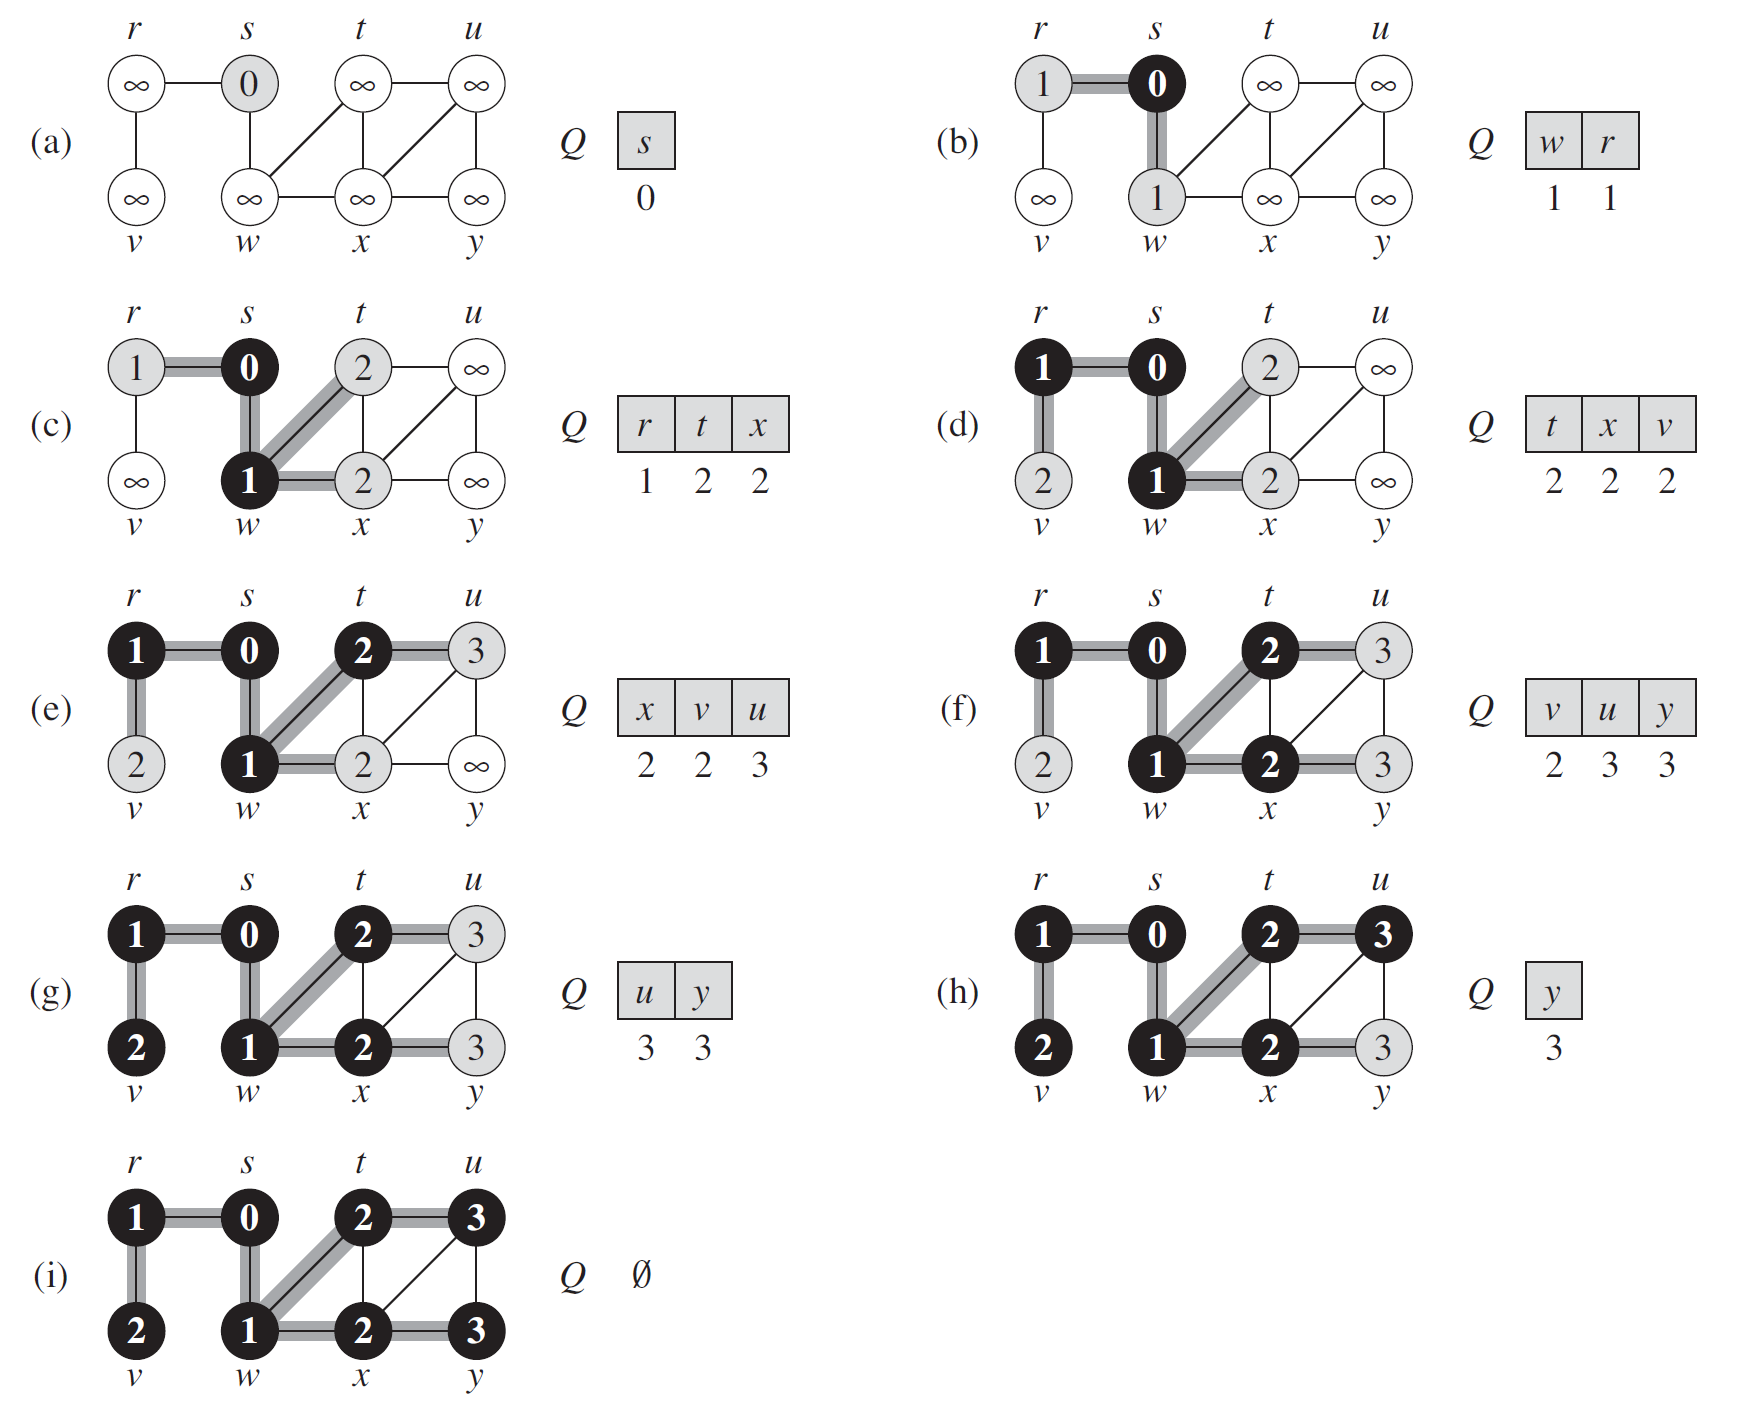
\includegraphics[scale=0.4]{Images/BFS-representation.png}
	\caption{نحوه اعمال شدن الگوریتم $BFS$}\label{Fig BFS representation}
\end{figure}


\newpage
\subsection{الگوریتم \lr{Greedy best-first search}}
ابتکار این روش این است که سعی می‌کند به سمت راسی که کمترین فاصله تا راس هدف دارد، گسترش پیدا کند، به امید آنکه به کوتاه‌ترین مسیر دست یابد \cite{russell2002artificial}. چون کمترین فاصله تا راس هدف را نداریم، حد پایین آن‌ را تقریب می‌زنیم و برابر فاصله قرار می‌دهیم. برای تقریب حد پایین، چون مختصات دو راس را داریم، کافی است طول خط راستی که راس را به راس هدف می‌رساند به دست آورد. در این راستا تابع $h(n)$ برای مختصات راس، \lr{n}، تعریف می‌گردد. اگر مختصات راس هدف با $n^\prime$ نمایش داده شود، مقدار تابع $h(n)$ که طول خط راست از راس تا راس هدف است به صورت زیر تعریف می‌گردد:
\begin{equation}\label{eq heuristic h}
h(n) = \|n - n^\prime\|_2
\end{equation}

مشخصا این روش نیز لزوما به جواب بهین نمی‌رسد، زیرا اصلا می‌تواند بین راسی که انتخاب شده تا راس هدف مسیری نباشد و به بن بست برسیم و مجبور به برگشت باشیم. همچنین برای مثال نقض نیز می‌توان نتیجه این روش را در بخش \ref{sec heuristic result} بررسی کرد که جواب آن بهین نیست.

در هنگام جست‌وجو در هر گام، والد هر راس را در درخت مسیر، به روز می‌گردد و در انتها با کمک از همین والد‌ها و با شروع از راس هدف، تا راس شروع، به عقب برمی‌گردیم. برعکس این مسیر، مسیری خواهد بود که ربات باید بپیماید.

\subsection{الگوریتم $A^*$}
الگوریتم $A^*$ ادامه‌ای بر الگوریتم \lr{Greedy best-first search} است که در آن علاوه بر تابع $h(n)$ که در رابطه \ref{eq heuristic h} تعریف شد، تابع $g(n)$ نیز تعریف می‌شود که مسافت واقعی بین نقطه شروع تا راس \lr{n} است. این فواصل با الگوریتم جست‌وجو مرتبا به روز می‌شود و در صورتی که مسیر کوتاه‌تری یافته شود نیز مقادیر آن به همراه مسیر واصله، به روز خواهند شد. همچنین برای یافتن کوتاه‌ترین مسیر نیز همانند الگوریتم \lr{Greedy best-first search}، برای هر راس یک والد در نظر گرفته شده است و با پیدا کردن مسیری کوتاه‌تر، مقداری کمتر برای تابع $g(n)$ در راس \lr{n}، والد نیز به راس جدیدی که به آن مسیر دارد، تغییر می‌یابد \cite{russell2002artificial}.

تابعی که طبق آن، راسی که کمترین مقدار آن را داشته باشد جست‌وجو خواهد شد، $f(n)$ می‌نامیم، که به صورت زیر تعریف می‌گردد:
\begin{equation}%\label{eq heuristic f}
	f(n) = g(n) + h(n)
\end{equation}

در نهایت نیز هنگامی که به راس هدف برسیم، الگوریتم جست‌وجو متوقف می‌گردد و سپس به طور بازگشتی از راس هدف، بر روی والدها به عقب برمی‌گردیم تا با عکس کردن جهت حرکت، مسیر ربات تعیین شود. 


\subsection{نتایج و مقایسه الگوریتم‌های ابتکاری}\label{sec heuristic result}
در این قسمت ابتدا به بررسی مسیر یافته شده توسط الگوریتم‌ها پرداخته می‌شود و سپس الگوریتم‌ها از نظر زمانی و ابعاد نقشه، مورد بررسی قرار می‌گیرند.

نقشه مورد استفاده برای بررسی پاسخ‌ها در شکل \ref{Fig mapRooz} آمده است. نقاط مشکی رنگ، مکانی هستند که مانع وجود دارد.
\begin{figure}[!h]
	\centering
	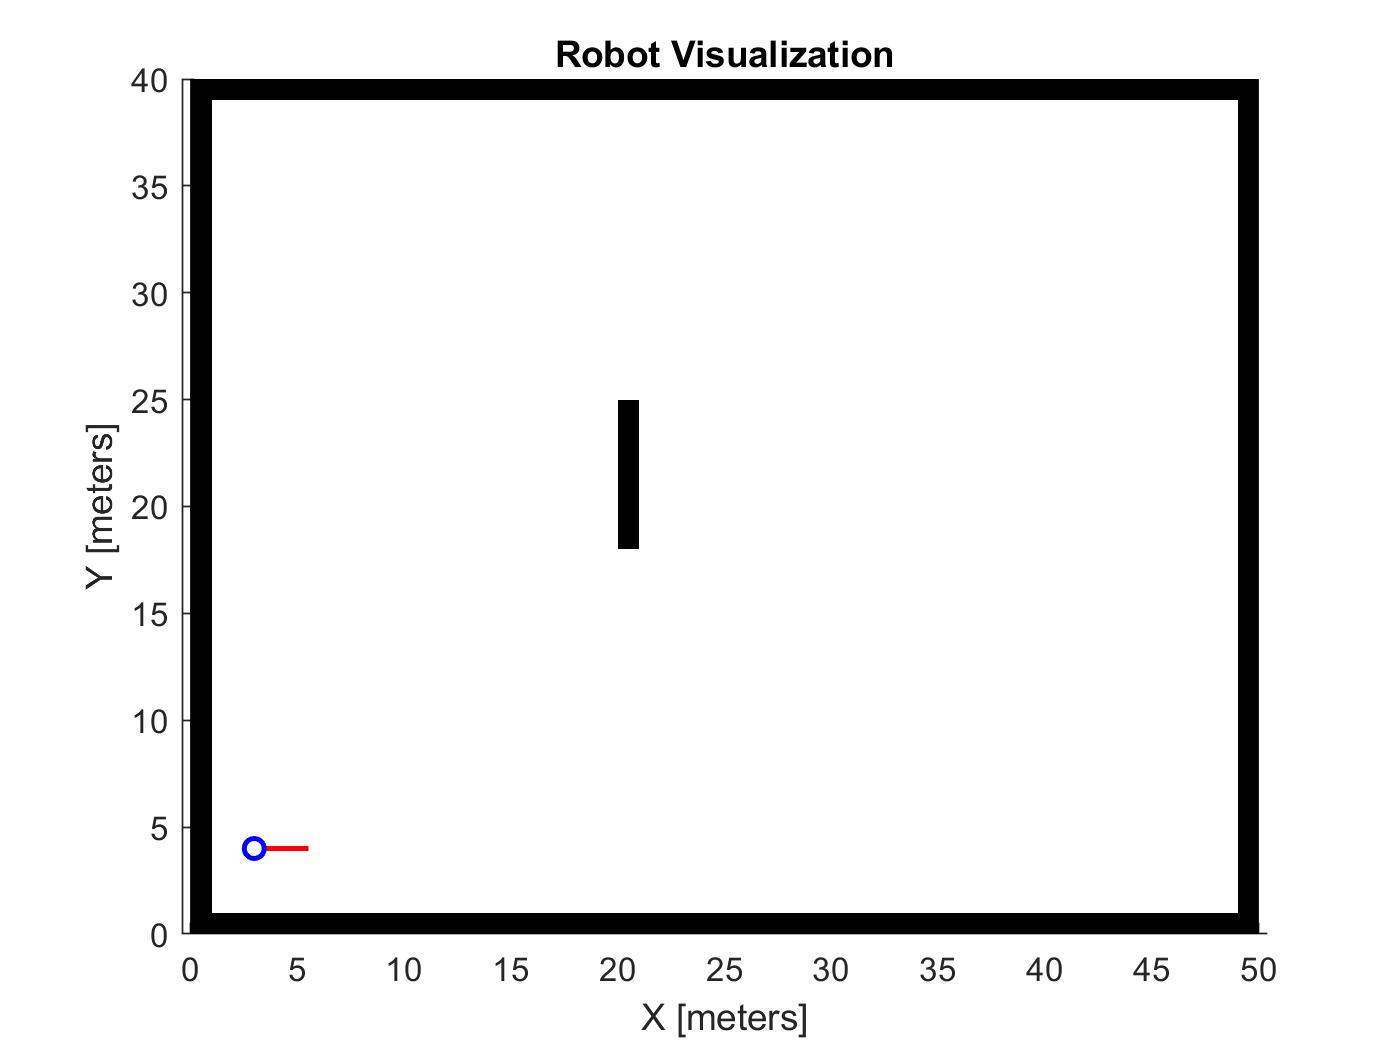
\includegraphics[scale=0.35]{Images/mapRooz.jpg}
	\caption{نقشه‌ای که الگوریتم‌ها به آن اعمال شده‌اند}\label{Fig mapRooz}
\end{figure}

حال برای هر سه الگوریتم، مسیری برای نقطه شروع $[6~~6]^T$ و هدف $[21~~24]^T$ خواسته شد. نتایج به شکل‌های \ref{Fig BFS path}، \ref{Fig Greedy path} و \ref{Fig A-star path} آمده است. نقاط ضربدر خورده قرمز، مسیر الگوریتم، و خط آبی مسیر پیموده شده توسط ربات هستند.
\begin{figure}[!h]
	\centering
	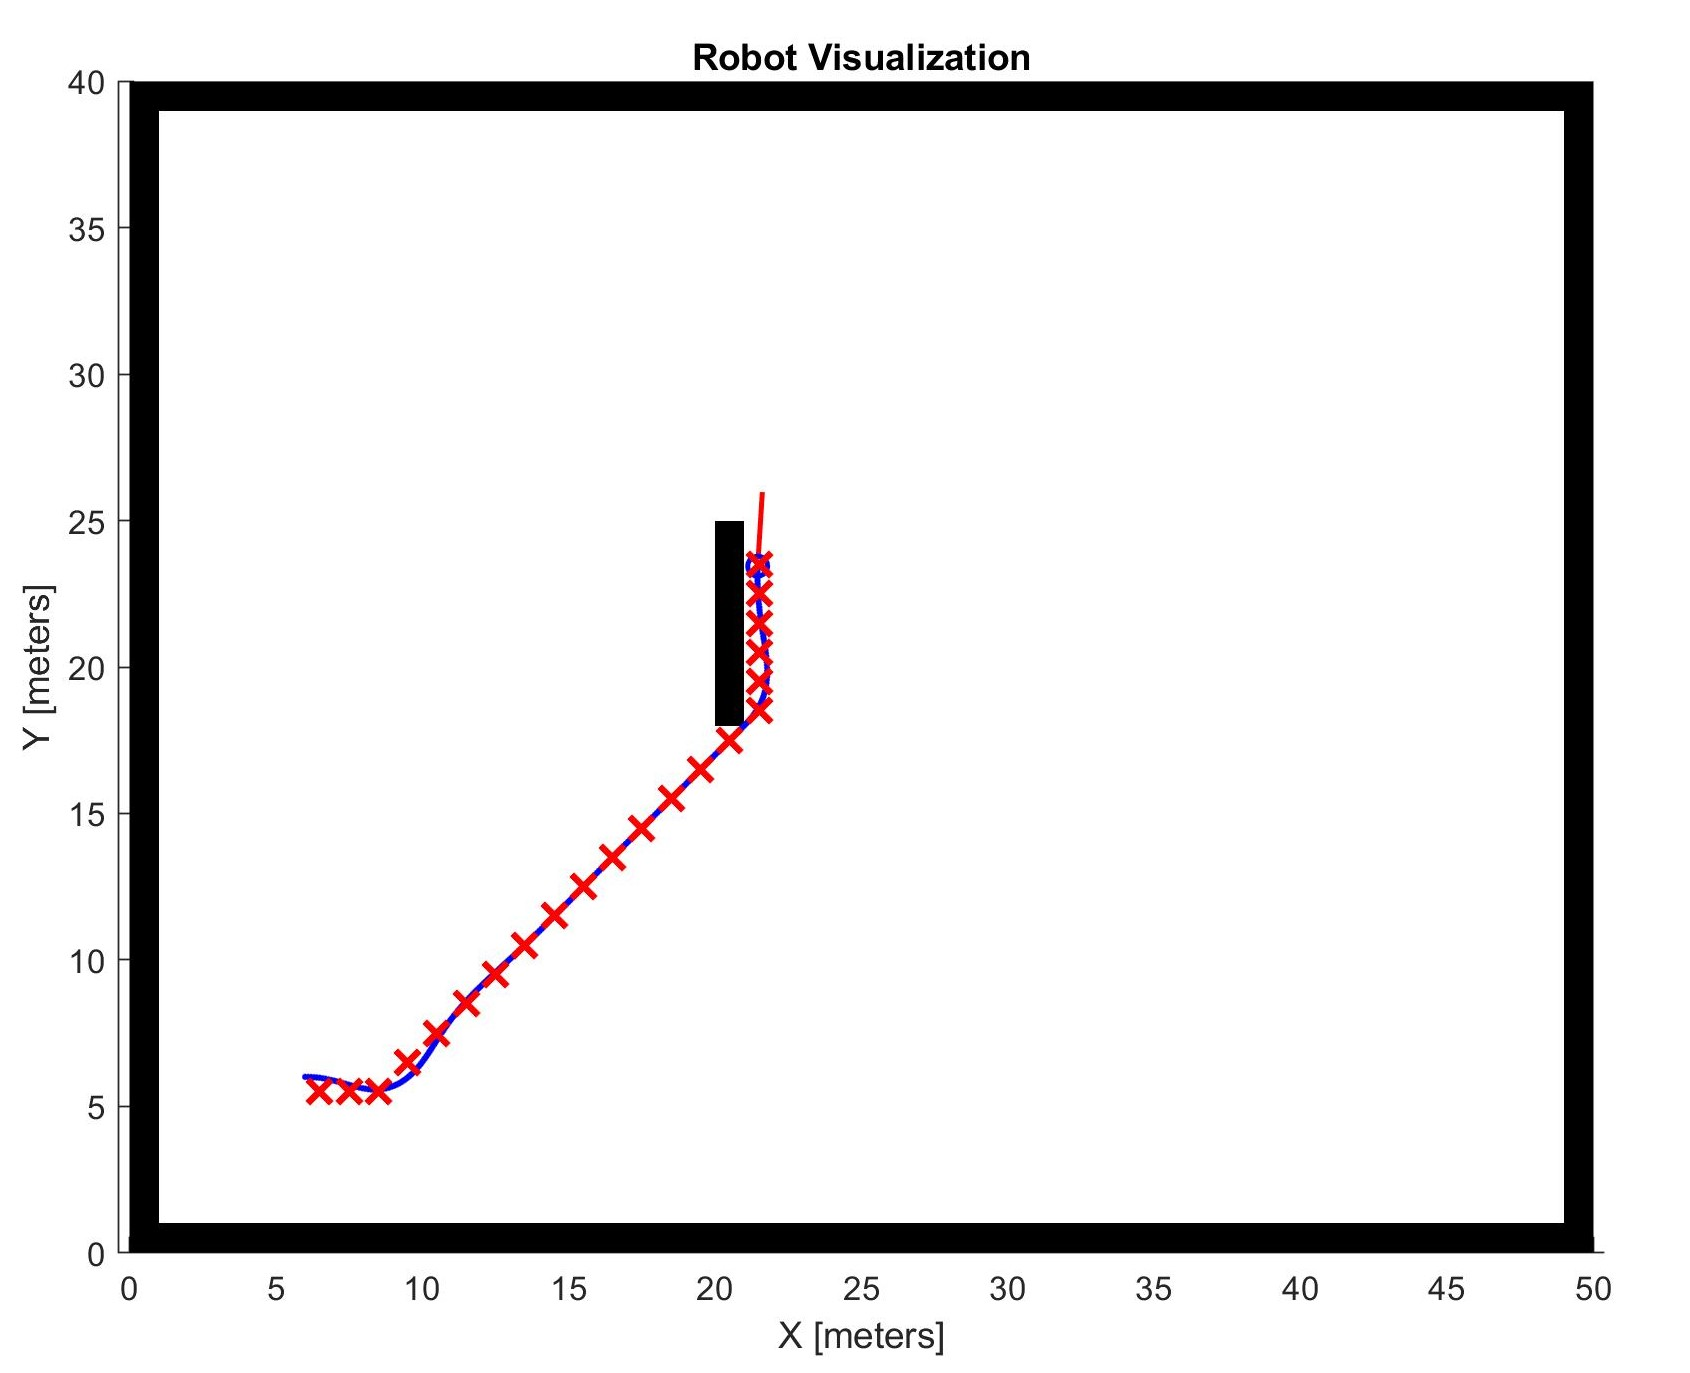
\includegraphics[scale=0.35]{Images/BFS path.jpg}
	\caption{مسیر پیشنهادی توسط الگوریتم \lr{BFS}}\label{Fig BFS path}
\end{figure}

\begin{figure}[!h]
	\centering
	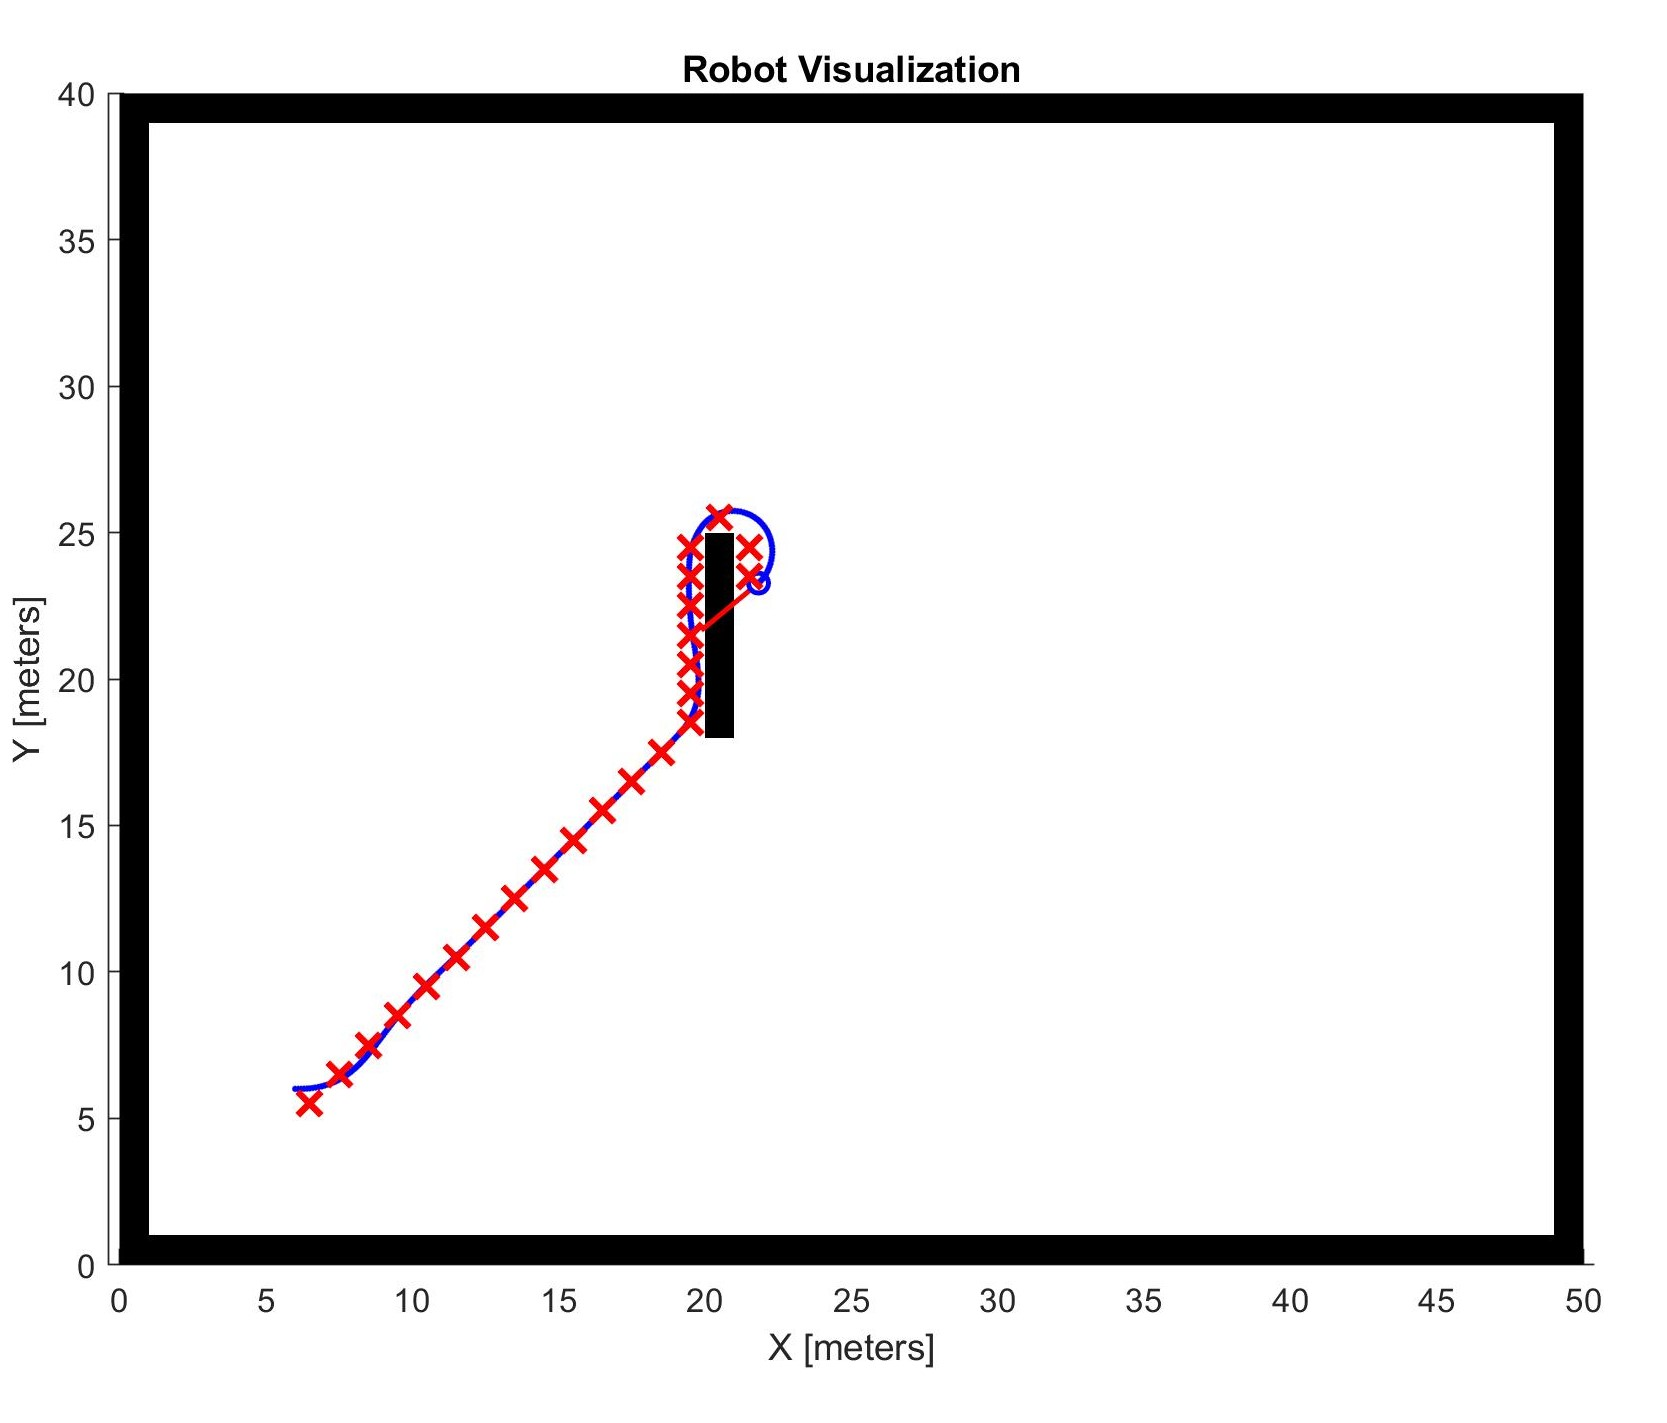
\includegraphics[scale=0.35]{Images/Greedy path.jpg}
	\caption{مسیر پیشنهادی توسط الگوریتم \lr{Greedy best-first search}}\label{Fig Greedy path}
\end{figure}

\begin{figure}[!h]
	\centering
	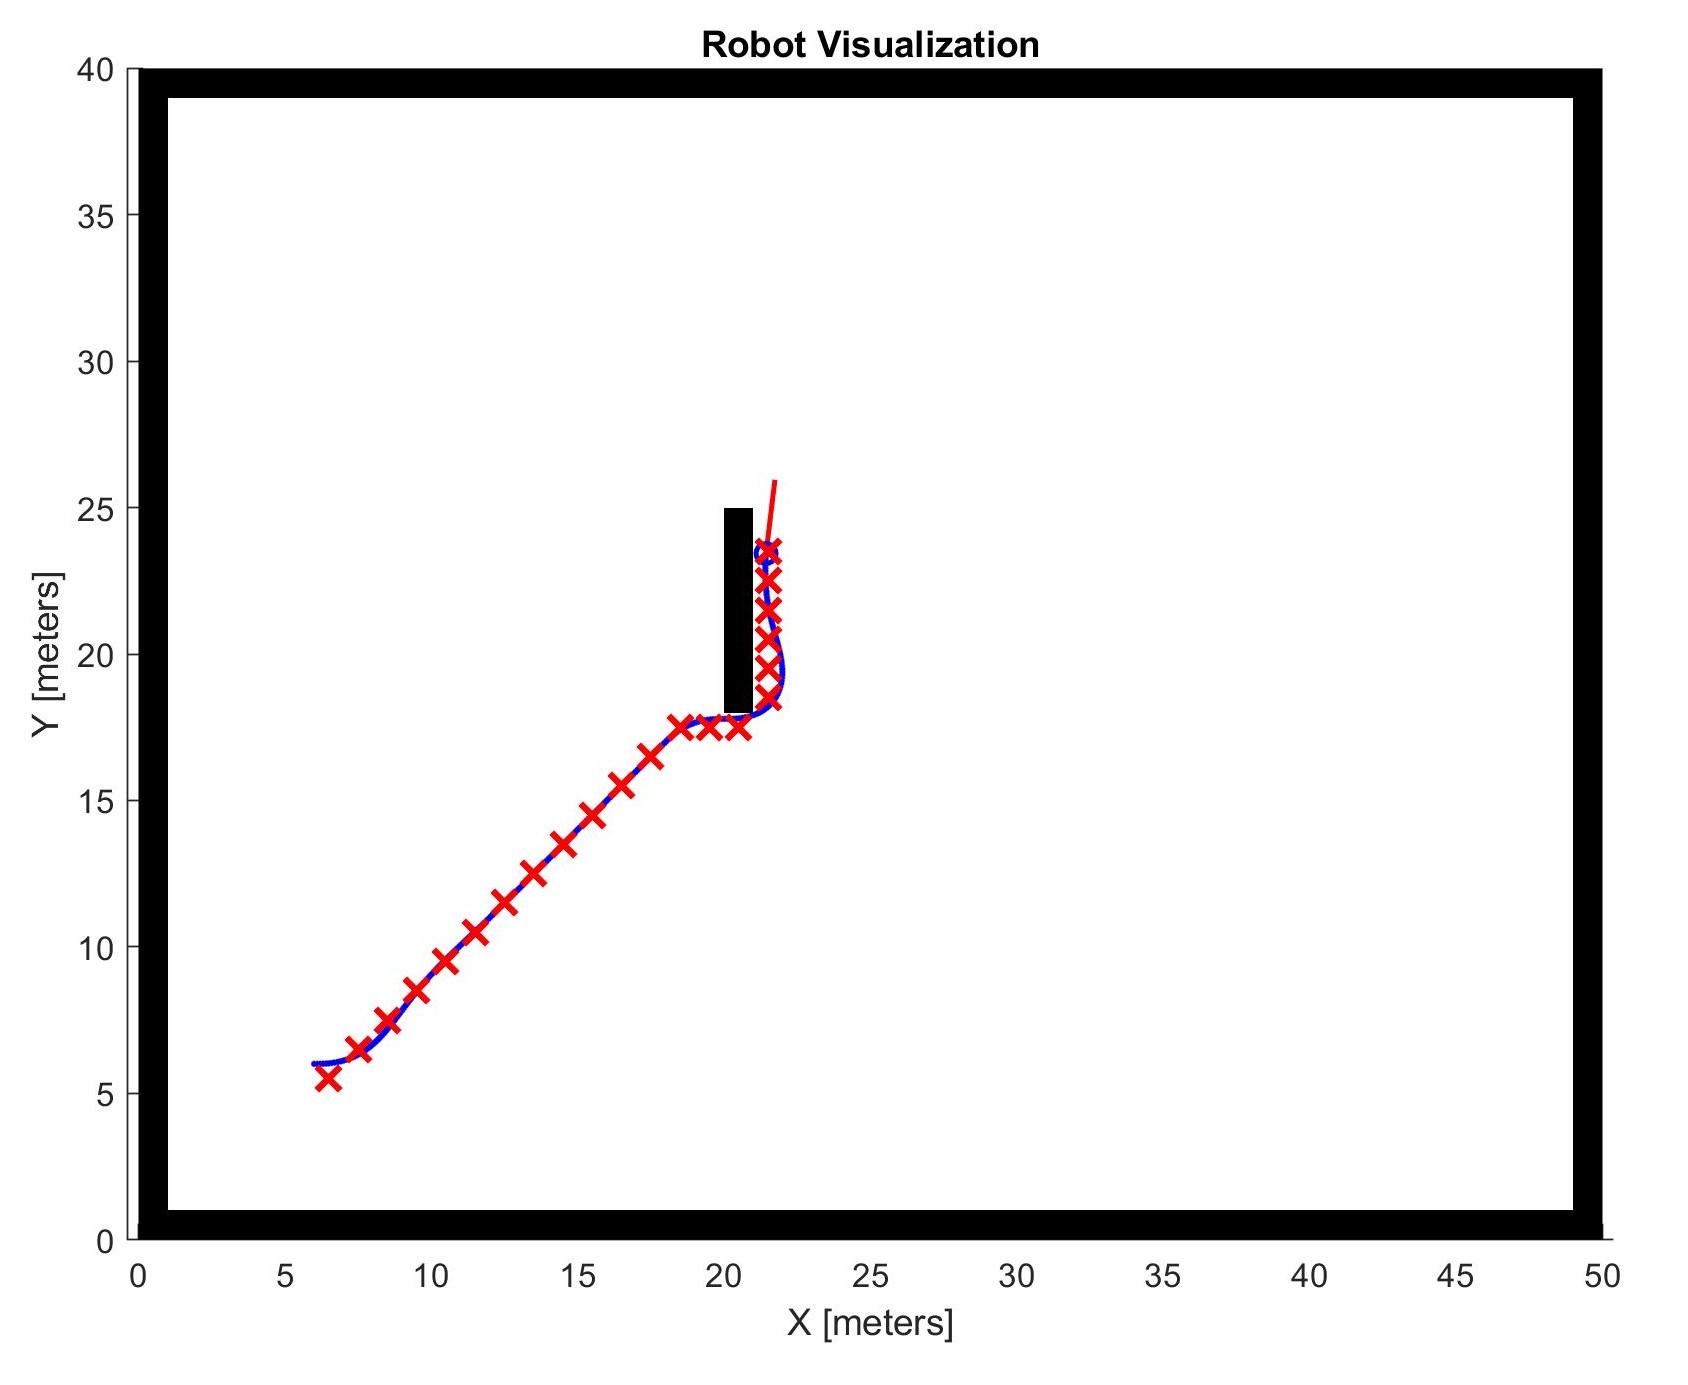
\includegraphics[scale=0.35]{Images/A-star path.jpg}
	\caption{مسیر پیشنهادی توسط الگوریتم $A^*$}\label{Fig A-star path}
\end{figure}

\newpage
همانطور که می‌شود دید در این مثال، الگوریتم، \lr{Greedy best-first search} مسیر طولانی‌تری نسبت به دو الگوریتم دیگر ارائه داده است. همچنین مسیرهای ارائه شده توسط دو الگوریتم، \lr{BFS} و $A^*$ هر دو بهین هستند.
\newpage
نکته دیگر قابل توجه، این است که هنگام چرخش به خصوص چرخش‌های سنگین همانند برگشت ربات در شکل \ref{Fig Greedy path} در بالای موانع، فشار زیادی به ربات آمده و کنترل مسیر برای او سخت بوده است. در نتیجه بهتر است کنترل‌کننده بهتری برای ربات در نظر گرفته شود. همچنین استفاده از الگوریتم‌هایی که سعی کنند میزان فشار وارده بر ربات را در تصمیمشان در نظر گرفته و کاهش دهند نیز، می‌تواند عضو کارهای آینده باشد.
\newpage
حال نوبت بررسی زمان مورد نیاز برای اجرای هر الگوریتم است. در این راستا، سه الگوریتم با نقاط تصادفی شروع و هدف، در حالی که برای هر سه یکسان باشند، اجرا گشتند. به ازای هر اندازه، 100 بار الگوریتم‌ها برای نقاط متفاوت بررسی و سپس از زمان آن‌ها میانگین گرفته شد. نتیجه در شکل \ref{Fig heuristic time} به نمایش در آمده است. همانطور که مشاهده می‌شود، زمان الگوریتم $A^*$ به مراتب بیشتر از الگوریتم‌های دیگر است. همچنین الگوریتم \lr{Greedy best-first search} کمترین زمان را دارد. در نتیجه هر چقدر بخواهیم به جواب معقولتری برسیم، مدت زمان بیشتر مورد نیاز است. در حالت کلی با توجه به اینکه برای 35000 نود، در کمتر از 200 میلی‌ثانیه برای الگوریتم $A^*$ به جواب رسیده است، استفاده از این الگوریتم توصیه می‌شود. قابل ذکر است که الگوریتم $A^*$ روش معقول‌تری نسبت به دو الگوریتم دیگر دارد و همچنین عملکرد آن در شرایطی که وزن‌ یال‌ها نسبت به هم بسیار متفاوت باشند بهتر نیز خواهد بود و قابلیت تعمیم به مسائل دیگر را نیز دارد.

\begin{figure}[!h]
	\centering
	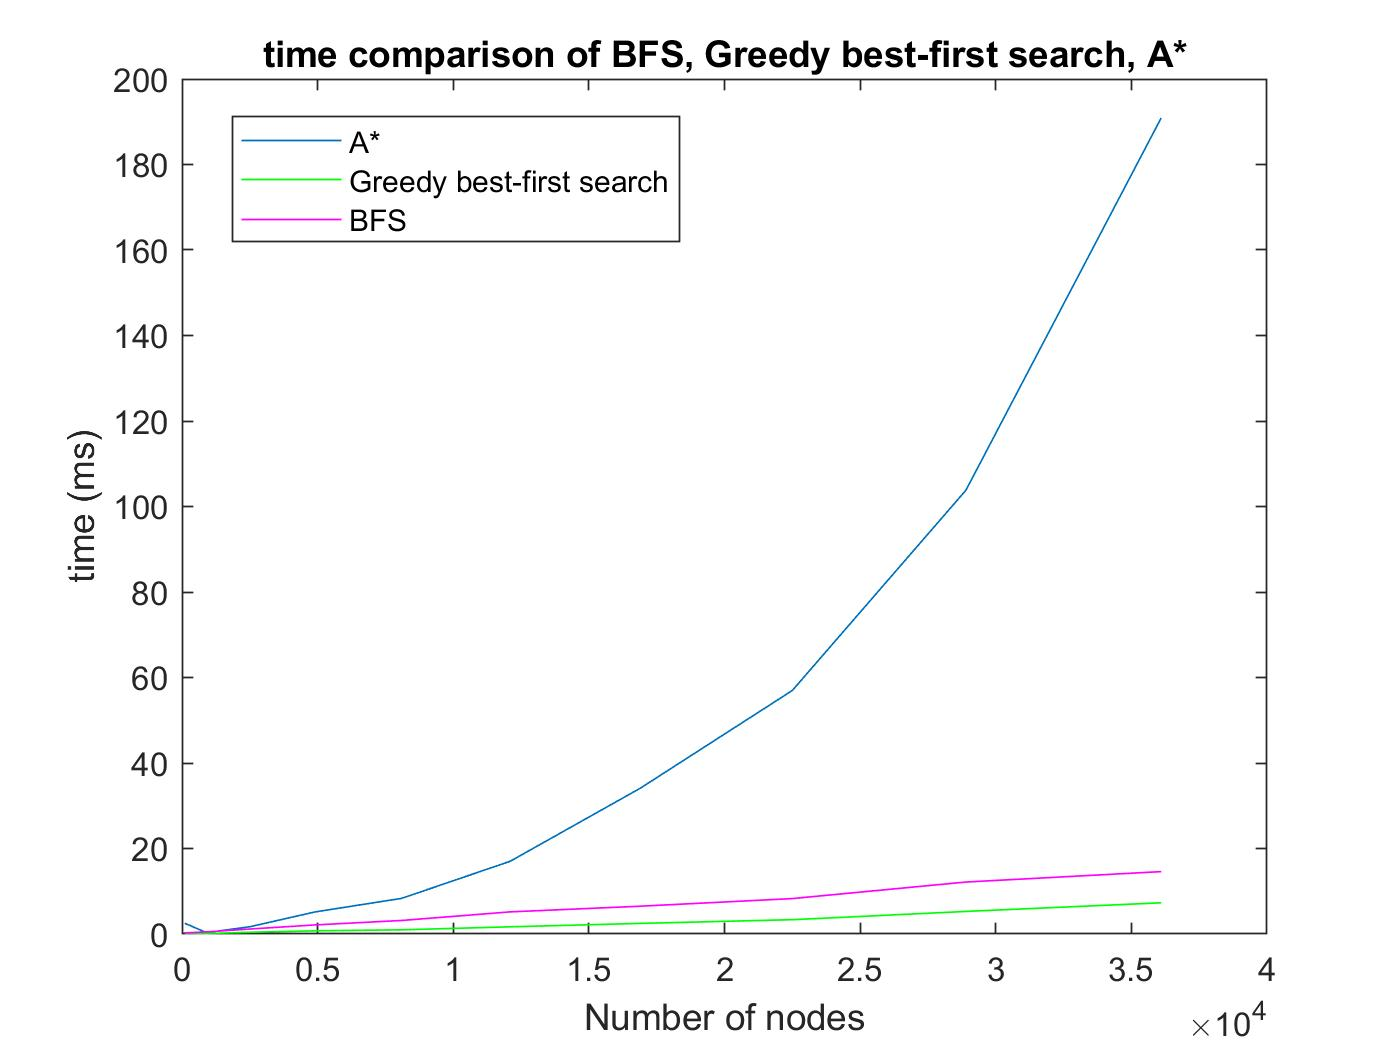
\includegraphics[scale=0.35]{Images/Heuristic time.jpg}
	\caption{مقایسه زمانی سه الگوریتم \lr{BFS}، \lr{Greedy best-first search} و $A^*$}\label{Fig heuristic time}
\end{figure}


\newpage
\section{\lr{Q-learning}}
\lr{Q-learning}
یک روش بدون مدل یادگیری تقویتی\LTRfootnote{reinforcement learning} است. همچنین می‌توان به آن به دید یک روش آسنکرون\LTRfootnote{asynchronous} برنامه ریزی داینامیک\LTRfootnote{dynamic programming (DP)} اشاره کرد \cite{watkins1992q}. محیط را همانند شرایط قبل نسبت به آن اطلاع کامل داریم. همچنین اقدامات ما نتایج قطعی\LTRfootnote{deterministic} دارند. حال به تعریف مجدد حالت‌ها و اقدامات می‌پردازیم. برای ساده‌سازی تمام مکان‌های عدد صحیح در محدوده کاری خود را به عنوان یک حالت در نظر گرفتیم. مجموعه \lr{A} که مجموعه اقدامات است به شرح زیر تعریف می‌شوند:
\begin{equation}\label{eq actions definition}
	A = \{[0~1]^T, [0~-1]^T, [1~0]^T, [-1~0]^T, [1~1]^T, [-1~1]^T, [1~-1]^T, [-1~-1]^T\}
\end{equation}
تنها نگته قابل توجه این است که در کناره‌های نقشه اگر از نقشه خارج می‌شدیم باید حالت بعدی را حذف نماییم. 

هدف کلی این روش دست یافتن به سیاست بهینه\LTRfootnote{optimal policy} از روی تابع \lr{Q} و ارزش هر حالت، \lr{V} طبق پاداش\LTRfootnote{reward} گرفته شده، است \cite{sutton1998introduction}. در ادامه به توضیح الگوریتم و روابط آن پرداخته می‌شود.

\subsection{الگوریتم \lr{Q-learning}}
با توجه به \cite{watkins1992q} تمام روابط برای حالت کلی‌تر که محیط غیرقطعی باشد نوشته شده است. لذا برای هر انتقال\LTRfootnote{transaction} یک احتمال در نظر گرفته شده است. در مسئله ما به دلیل اینکه محیط قطعی است، احتمال برای یک حالت 1 و بقیه حالت‌ها صفر خواهد شد. در نتیجه از نوشتن آن خودداری شده است. ارزش هر حالت بر طبق سیاست $\pi$ به صورت زیر تعریف می‌گردد:
\begin{equation}
	V^\pi (x) \equiv R_x(\pi(x)) + \gamma V^\pi (y)
\end{equation}
که در آن \lr{y} حالتی است که از حالت \lr{x} طبق سیاست $\pi$ به آن خواهیم رسید. همچنین نسبت ارزشی که \lr{s} گام قبل‌تر گذاشته شده نسبت به ارزش الان، $\gamma^s$ برابر است 
($0 < \gamma < 1$).

در نتیجه برای سیاست بهینه $\pi^*$ خواهیم داشت:
\begin{equation}
	V^*(x) \equiv V^{\pi^*} (x) = \max_{a}\{R_x(a) + \gamma V^{\pi^*} (y)\}
\end{equation}

حال عبارتی که باید از آن نسبت به هر اقدام، ماکزیمم گرفته شود را تابع \lr{Q} تعریف می‌کنند.
\begin{equation}
Q^\pi (x,~a) = R_x(a) + \gamma V^\pi (y)
\end{equation}

حال در گام \lr{n}، هر حالت و اقدام مطابق روابط \ref{eq updating Q} و \ref{eq updating V} توابع \lr{Q} و \lr{V} به روزرسانی می‌گردند.
\begin{equation}\label{eq updating Q}
Q_n(x,~a) = (1-\alpha_n)Q_{n-1}(x,~a) + \alpha_n[r_n + \gamma V_{n-1}(y_n)]
\end{equation}
که در آن داریم:
\begin{equation}\label{eq updating V}
V_{n-1}(y) \equiv \max_{b}\{Q_{n-1}(y,~b)\}
\end{equation}

\subsection{پیاده‌سازی الگوریتم \lr{Q-learning}}
به دو روش متفاوت الگوریتم \lr{Q-learning} پیاده‌سازی و در \cite{roozbeh2020} قابل دسترسی است. در روش اول از برنامه ریزی دینامیک استفاده نشده است و با شروع از مکان اولیه ربات، به صورت رندوم، به حالت‌های مجاور رفته و به روز رسانی انجام شده است. در روش دوم از برنامه‌ریزی دینامیک استفاده شده است. چون در برنامه‌ریزی دینامیک هدف این است که با اندکی افزودن به پیچیدگی حافظه استفاده شده، از پیچیدگی زیاد زمانی بپرهیزیم، در روش اول، محاسبات بسیار طولانی بودند، به نحوی که حتی پاسخ‌ها هم تفاوت زیادی تا پاسخ بهینه داشتند. اما در روش دوم، به صورت گام به گام، هر بار تمام حالت‌ها و اقدامات بررسی و به روزرسانی می‌شدند و با بررسی بیشترین تغییر، اگر از حد تعیین شده کمتر می‌شد الگوریتم متوقف می‌گشت. لذا دید خوبی نیز نسبت به شرایط الگوریتم و مقدار بهینگی به دست می‌آمد و از محاسبات اضافی جلوگیری می‌شد.

نکته مهم در این الگوریتم، تنظیم کردن\LTRfootnote{tuning} مقدار $\alpha$ و $\gamma$ و همچنین تعیین یک پاداش مناسب $r$ می‌باشد. در بخش بعد به خصوص در مورد انتخاب‌های پاداش، صحبت خواهد شد.

\subsection{نتایج مسیریابی با \lr{Q-learning}}
در ابتدا نتیجه روش‌های اول و دوم بررسی شده و سپس بعد از مشخص شدن بررسی روش دوم، پاداش‌های متفاوت برای روش دوم بررسی خواهند شد. نتیجه روش اول برای یک میلیون بار شروع و رسیدن به نقطه هدف یا مانع  در شکل \ref{Fig QL random} آمده است.
\begin{figure}[!h]
	\centering
	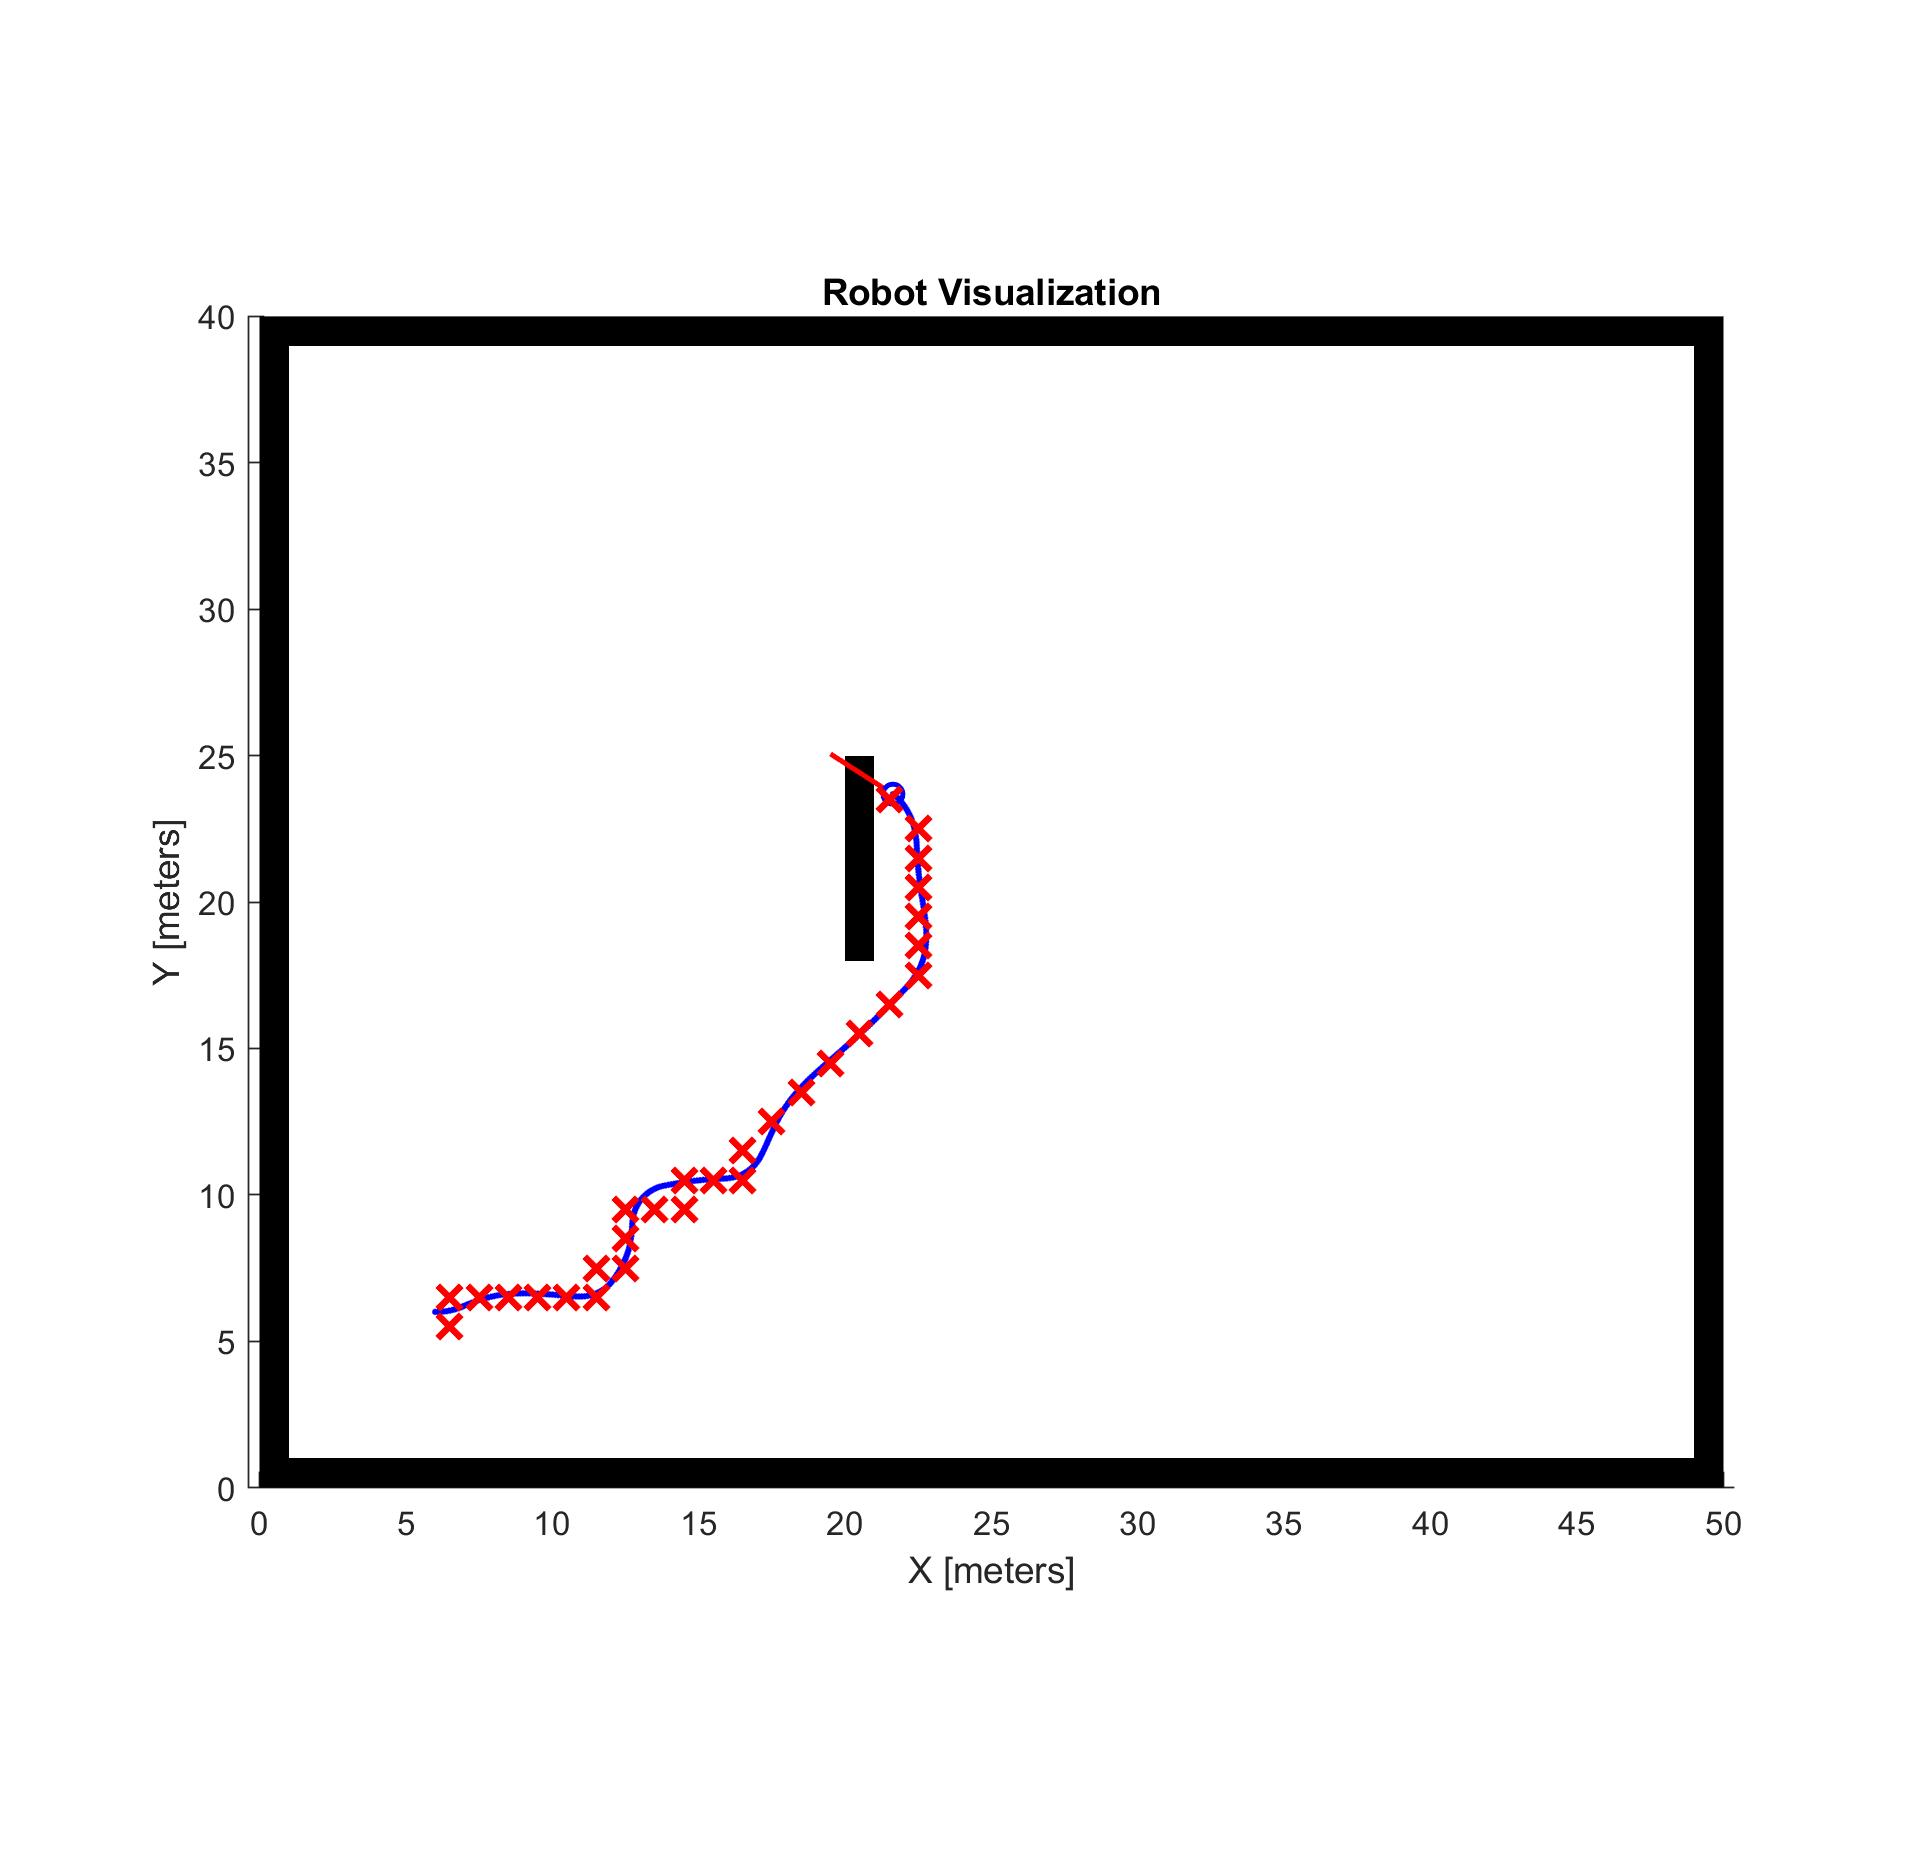
\includegraphics[scale=0.35]{Images/QL path.jpg}
	\caption{نتیجه الگوریتم \lr{Q-learning} برای یادگیری تصادفی}\label{Fig QL random}
\end{figure}

همانطور که مشخص است زمان مورد نیاز برای یک میلیون پردازش بسیار زیاد است و یک ضعف دیگر این الگوریتم یادگیری این است که بسیار طول می‌کشد تا به پاسخ صحیح دست یابد. با روش برنامه‌ریزی داینامیک برای الگوریتم یادگیری، نتایج بسیار بهتری از نظر زمانی و بهینگنی به دست آمد. همچنین این الگوریتم سیاست بهینه را برای تمامی نقاط محاسبه می‌کند. در ادامه این پاسخ‌ها بررسی خواهند شد.

همانطور که گفته شد، با داشتن بیشترین تغییر در مقادیر \lr{V} یک معیار خوب برای درجه یادگیری الگوریتم وجود دارد. حال توابع مختلف پاداش را بررسی می‌گردد. در همه توابع اگر مدل به حالت هدف برسد با مقدار $R=10$ پاداش می‌گیرد و اگر به موانع بخورد یا از صفحه خارج شود به مقدار $R=-10$ جریمه می‌شود. در شکل \ref{Fig QL R=-1} نتیجه مسیریابی با $R=-1$ به ازای بقیه حالت‌ها نشان داده شده است. دلیل این مقدار دهی این است که ربات سعی کند با کمترین اقدام به حالت هدف برسد. این مسیریابی بعد از 76 گام به نتیجه رسیده است.
\begin{figure}[!h]
	\centering
	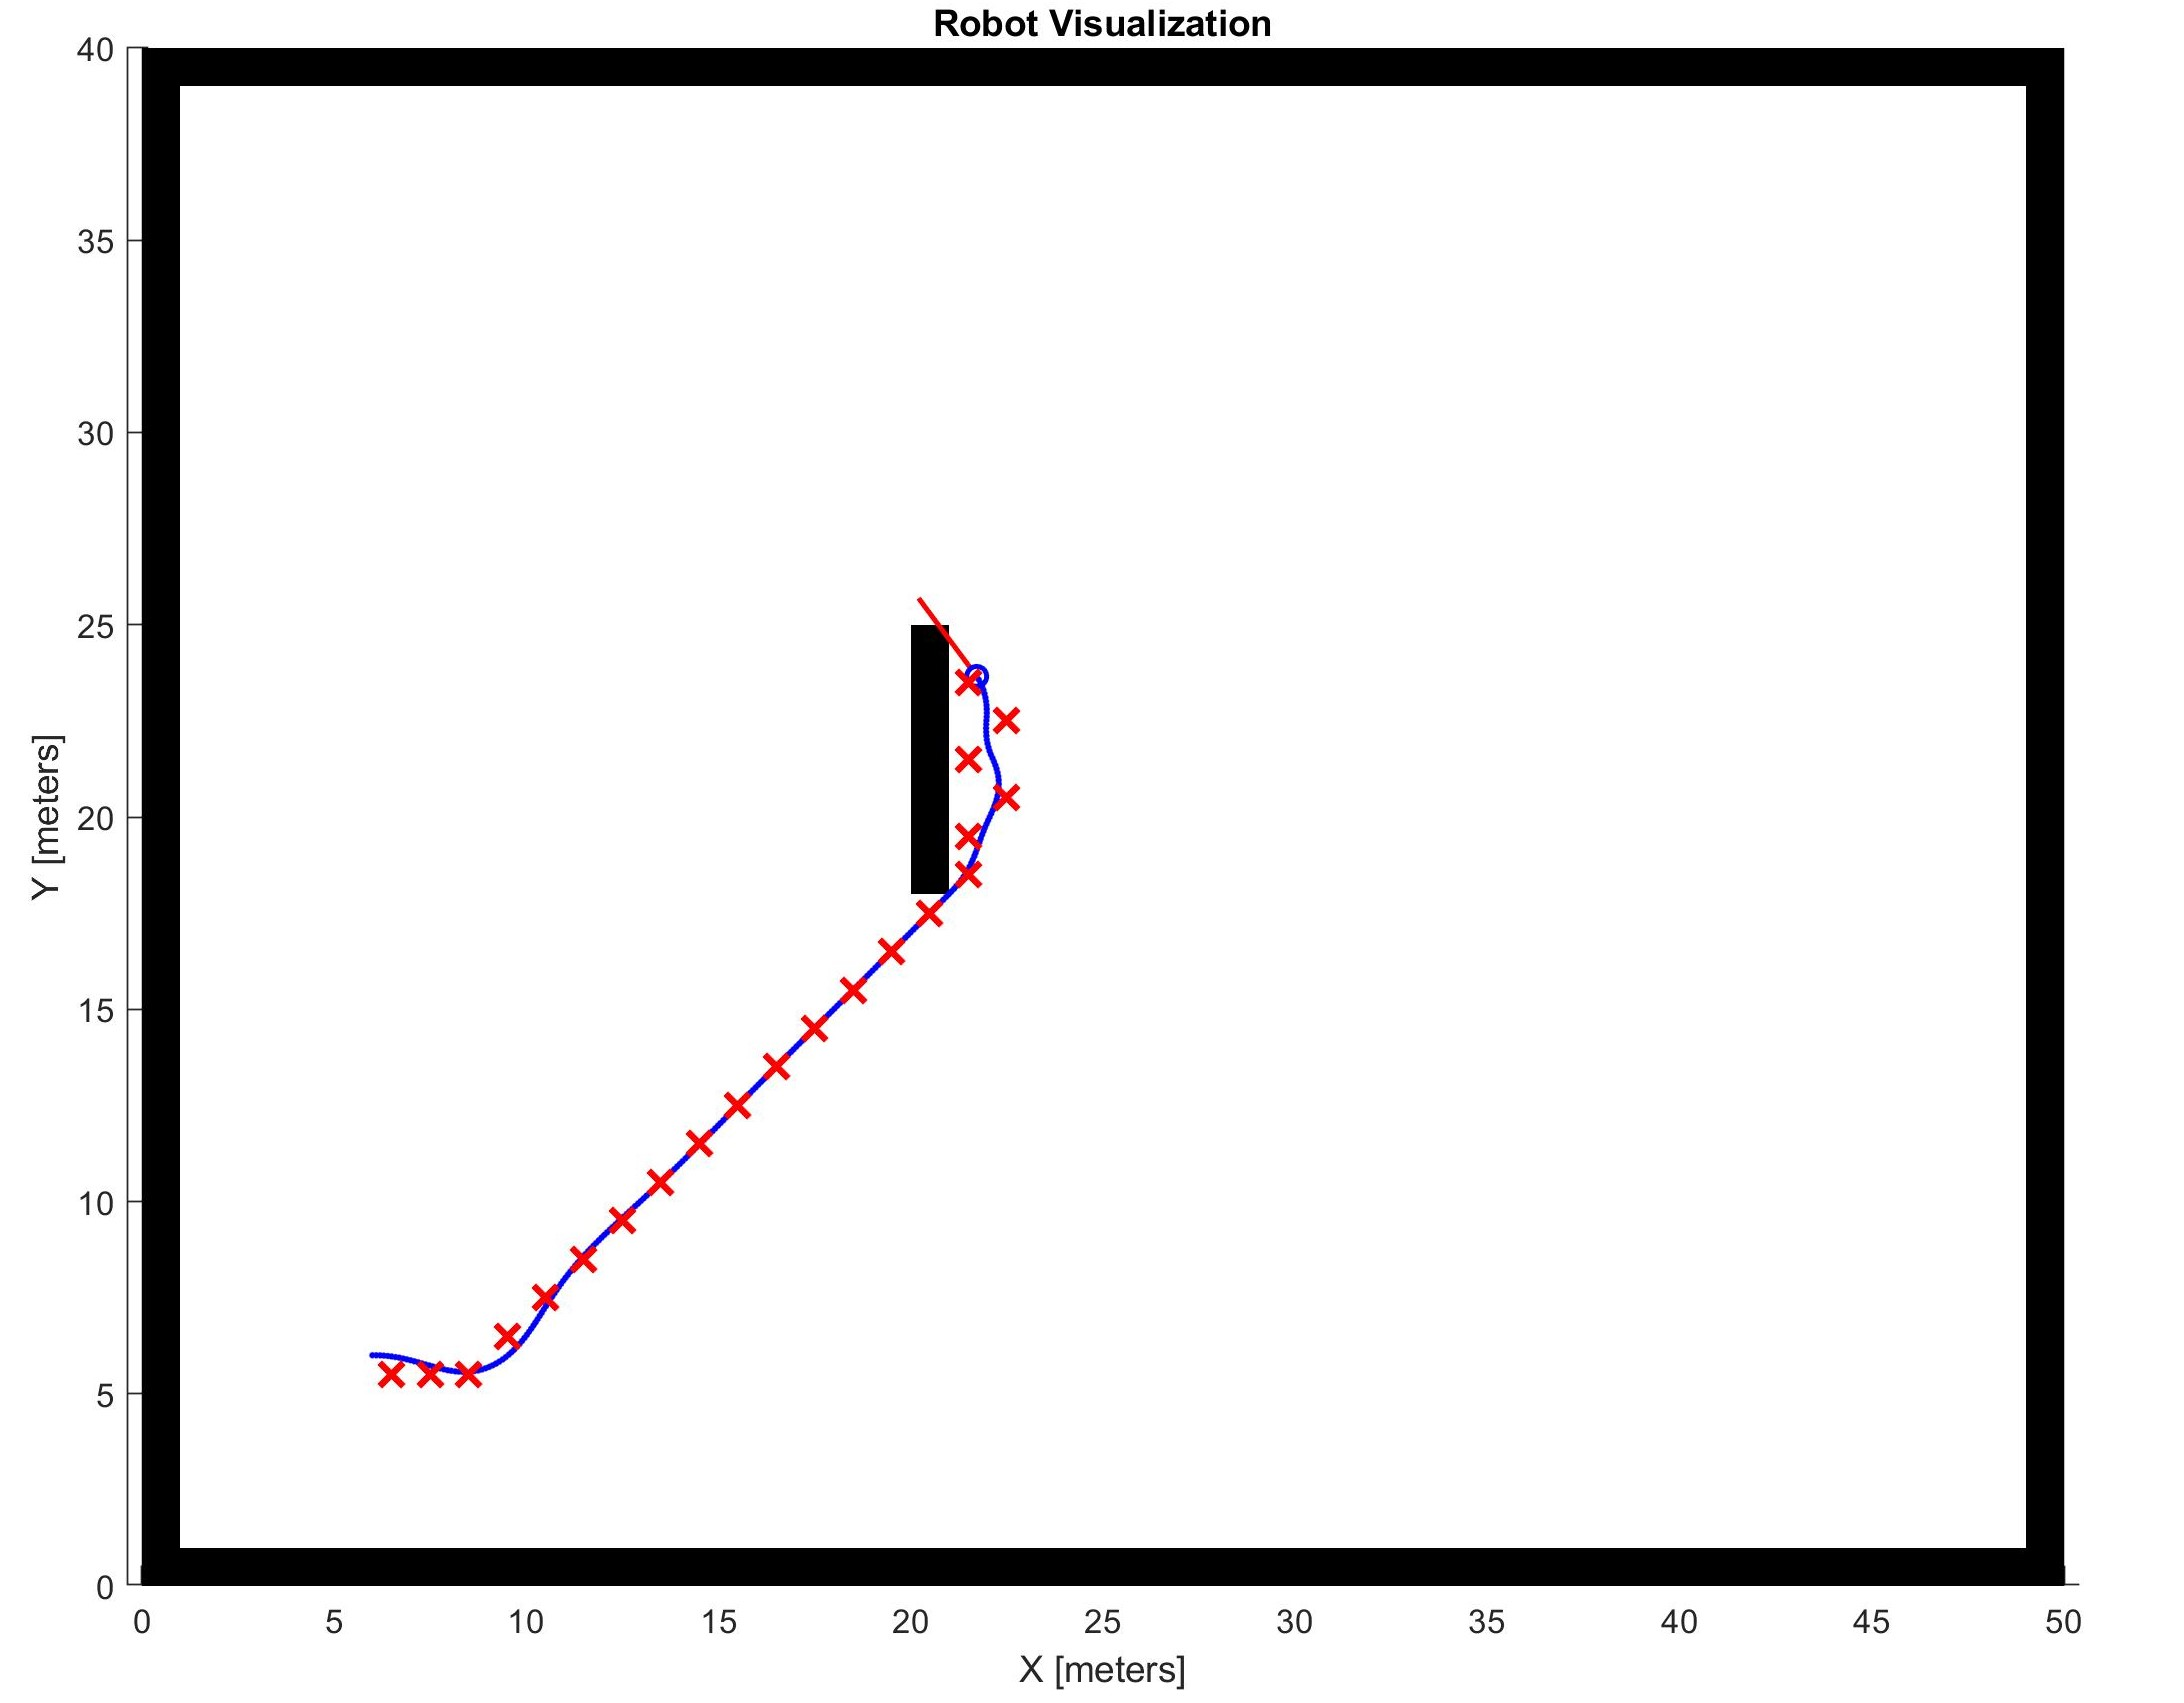
\includegraphics[scale=0.3]{Images/QL path R=-1.jpg}
	\caption{نتیجه الگوریتم \lr{Q-learning} برای یادگیری با $R=-1$}\label{Fig QL R=-1}
\end{figure}

همانطور که دیده می‌شود در انتها مسیریابی زیگ زاگ شده است. دلیل این مسئله این است که اگر ربات به صورت مستقیم حرکت کند یا زیگ زاگ، از نظر تعداد اقدام‌ها جریمه‌ای متفاوت دریافت نخواهد کرد. برای اینکه ربات تفاوت میان حرکت مستقیم یا زیگ زاگ را درک کند باید توجه کنیم که هدف ما تعداد اقدامات نیست بلکه مسافت پیموده شده است . لذا طبق رابطه \ref{eq actions definition} برای هر اقدام جریمه‌ای برابر با $R=-\|a\|_2$ در نظر می‌گیریم که برابر با مسافت پیموده شده تحت هر اقدام است. در نتیجه هدف مینیمم کردن مسیر پیموده شده است. نتیجه این روش در شکل \ref{Fig QL R=-normA} بعد از 79 گام به نمایش در آمده است.
\begin{figure}[!h]
	\centering
	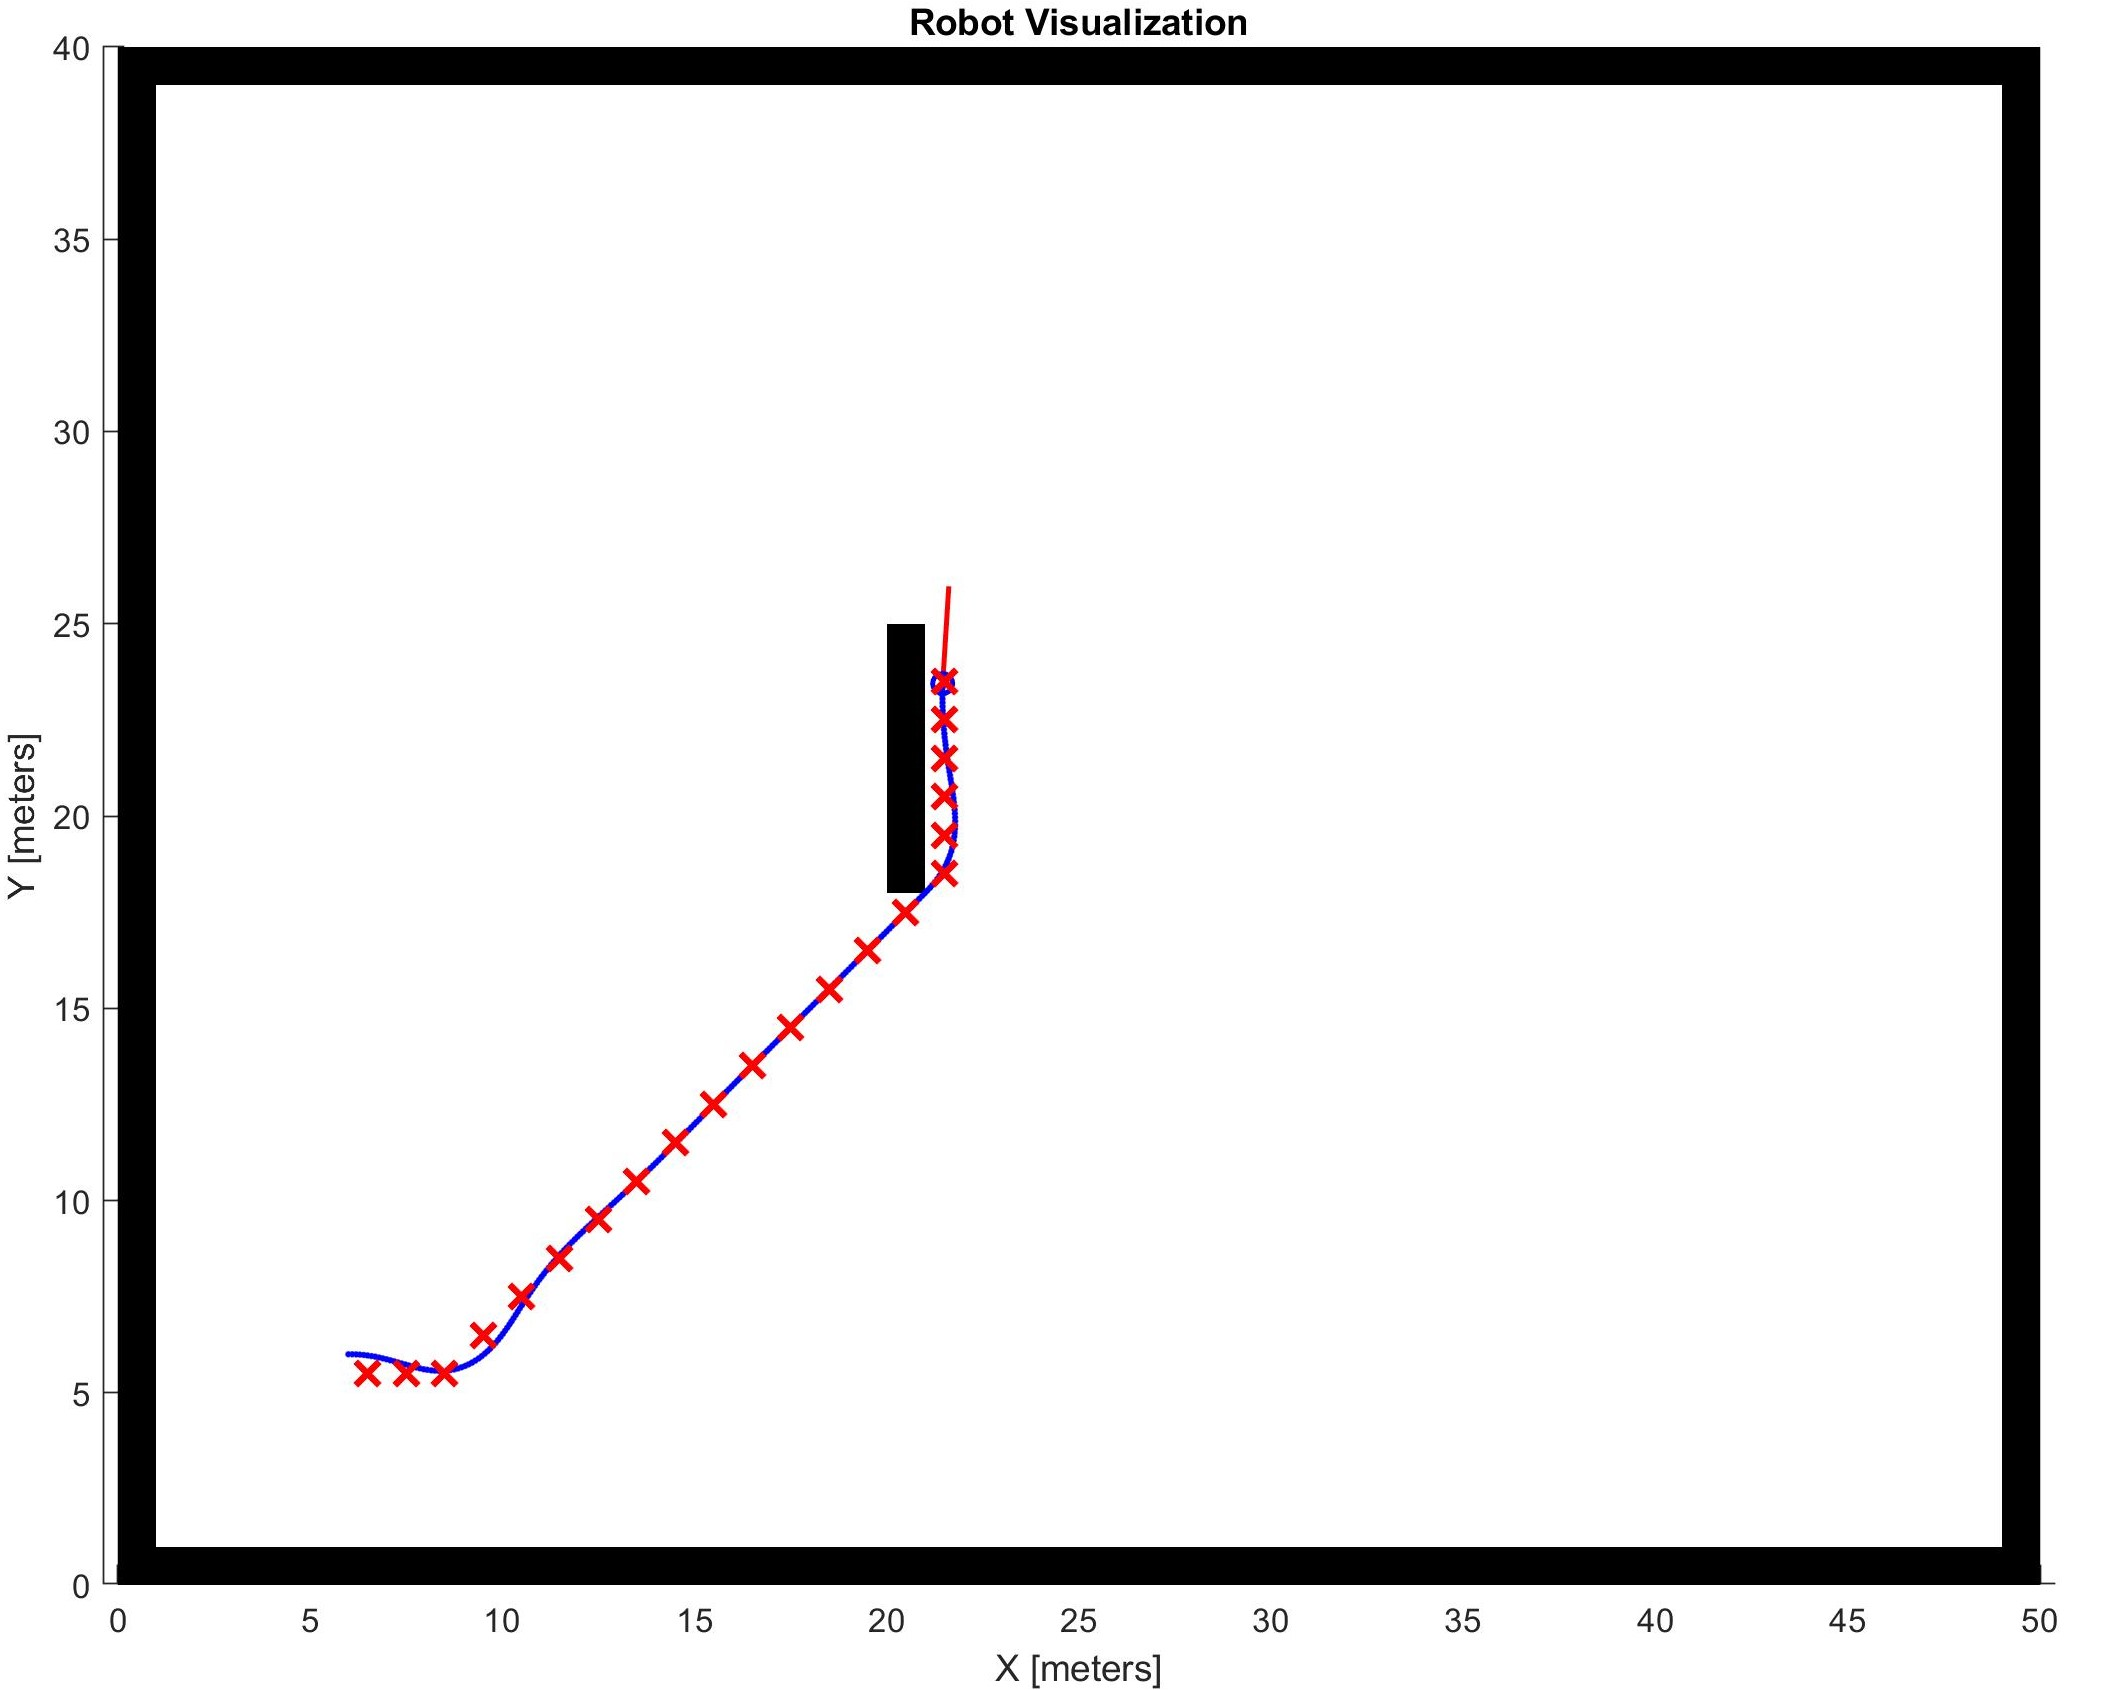
\includegraphics[scale=0.3]{Images/QL path R=-normA.jpg}
	\caption{نتیجه الگوریتم \lr{Q-learning} برای یادگیری با $R=-\|a\|_2$}\label{Fig QL R=-normA}
\end{figure}

در نتیجه مقداردهی پاداش و جریمه به صورت 
\begin{equation}\label{eq R optimal}
	R=-\|a\|_2
\end{equation}

بهترین روش انتخاب است و با زمان کافی به پاسخ بهین خواهد رسید. در ادامه پروژه نیز از آن استفاده خواهد شد. حال به تعدادی از اشتباهات ممکن در مقداردهی \lr{R} پرداخته خواهد شد.

\subsection{اشتباهات رایج در انتخاب پاداش}
در ابتدا مفهوم این مطلب در بازی شطرنج مثال زده خواهد شد و سپس به مسئله این پایان‌نامه پرداخته خواهد شد.

اگر برای یادگیری شطرنج توسط یک مدل هدف نهایی که مات کردن حریف و پیروزی است را پاداش بگیریم اما در کنارش به بردن مهره‌ها هم امتیاز دهیم، امکان دارد مدل به جای تمرکز بر پیروزی بیشتر دنبال گرفتن مهره‌های حریف باشد مخصوصا اگر پاداش پیروزی به نسبت گرفتن مهره‌ها بسیار بزرگ نباشد و گرفتن مهره نسبت به پیروزی برای او اهمیت بیشتری داشته باشد. یا حتی تنها پیروزی را عقب بیاندازد تا مهره‌های بیشتری را بگیرد و سپس اقدام به بردن بازی نماید و در این بین توسط حریف شکست بخورد هر چند انتخاب این مدل تابع هدف باعث دیدن نتایج اولیه بهتری از سوی 

این اشتباهات امکان دارد در مسیریابی برای ربات هم اتفاق بیفتد. به عنوان مثال اگر طبق فاصله حالت بعدی تا نقطه هدف جریمه انجام گردد، $R=-\frac{\|(y-goal)\|_2}{1000}$، مسیریابی بهین نخواهد بود و در این مثال همانطور که در شکل \ref{Fig QL R=-normpos-goal} مشخص است، تحت تغییر مسیر ناگهانی ربات با مانع اثابت کرده است. دلیل این انتخاب این بوده که حالت $[19~~19]^T$ جریمه کمتری داشته و ربات علاقه‌مند به عبور از آن بوده و همچنین روی مسافت پیموده شده جریمه‌ای تعیین نشده است. هر چند سریع‌تر و با 77 گام به پاسخ رسیده است. دلیل تقسیم بر 1000 نیز ایجاد نسبت معقول بین پاداش رسیدن و جریمه بوده است.
\begin{figure}[!h]
	\centering
	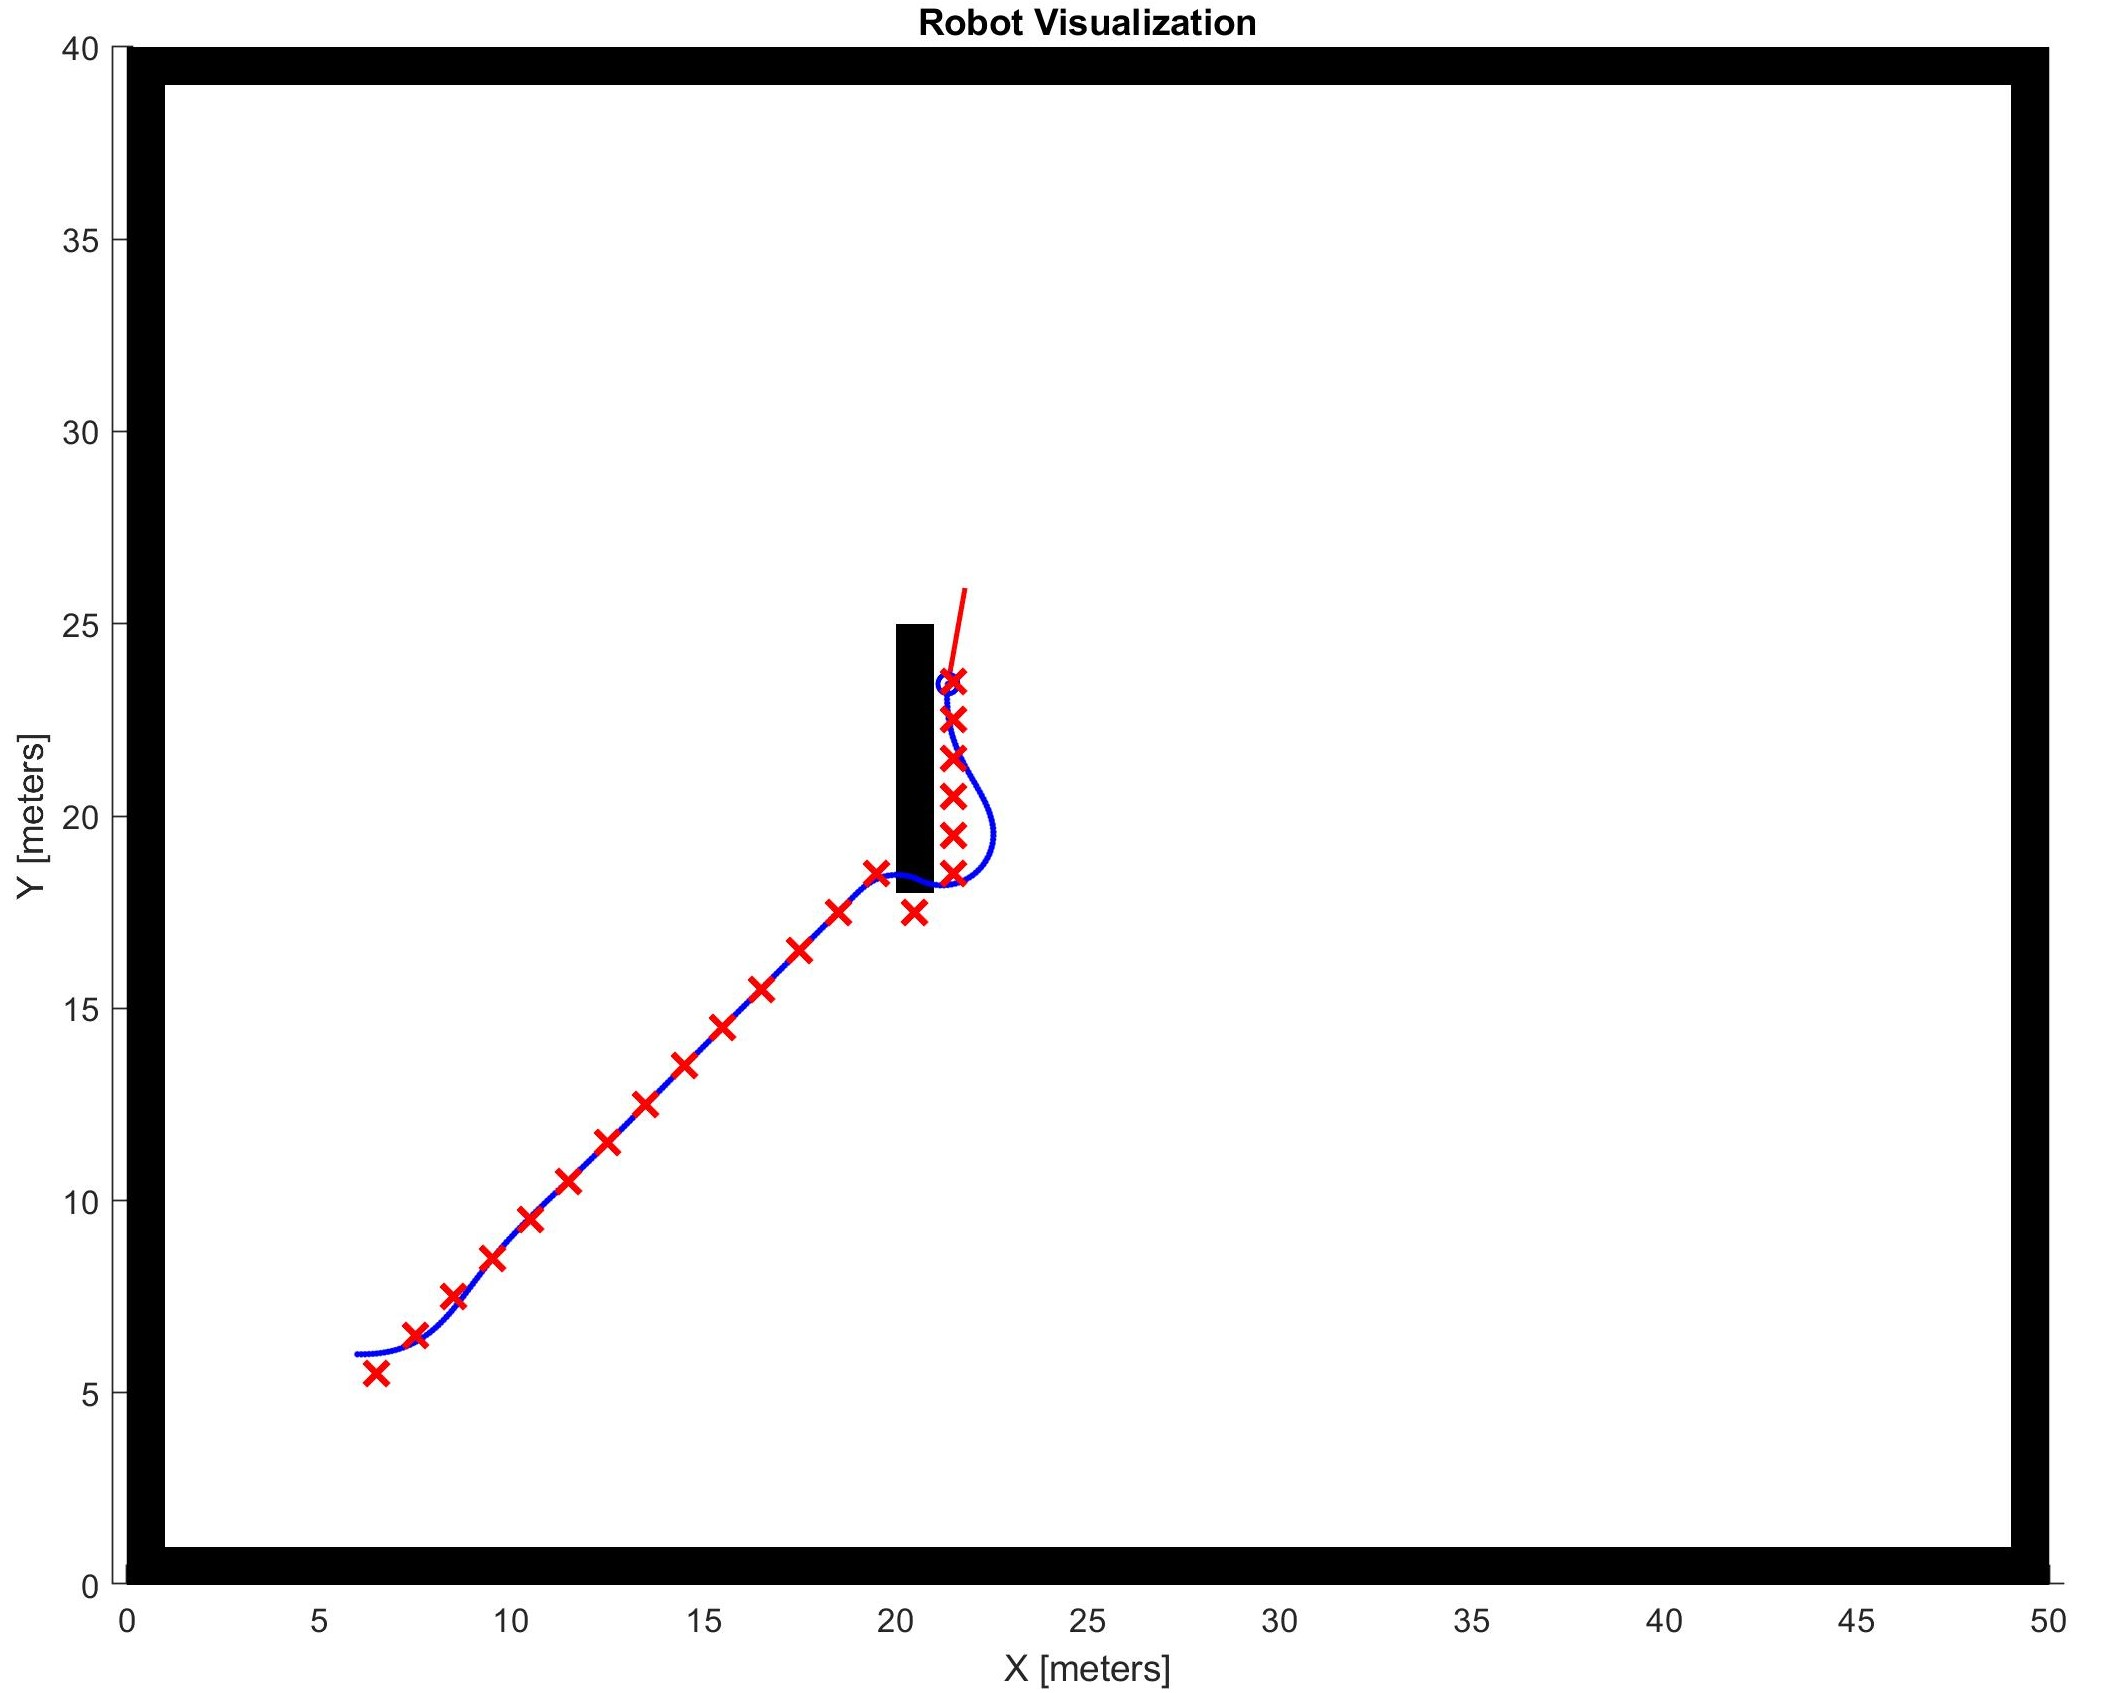
\includegraphics[scale=0.3]{Images/QL path R=-normpos-goal.jpg}
	\caption{نتیجه الگوریتم \lr{Q-learning} برای یادگیری با $R=-\frac{\|(y-goal)\|_2}{1000}$}\label{Fig QL R=-normpos-goal}
\end{figure}

حتی اگر بیاییم و تابع پاداشی تعریف کنیم که بسیار نزدیک به تابع پاداش بهین \ref{eq R optimal} باشد، مجددا شکست خواهیم خورد. در این قسمت اگر پاداش را برابر مقدار فاصله‌ای بگیریم که به نقطه هدف نزدیک شده‌ایم باز ربات به پیچ سخت همانند حالت قبل تصادف خواهد کرد.
\begin{figure}[!h]
	\centering
	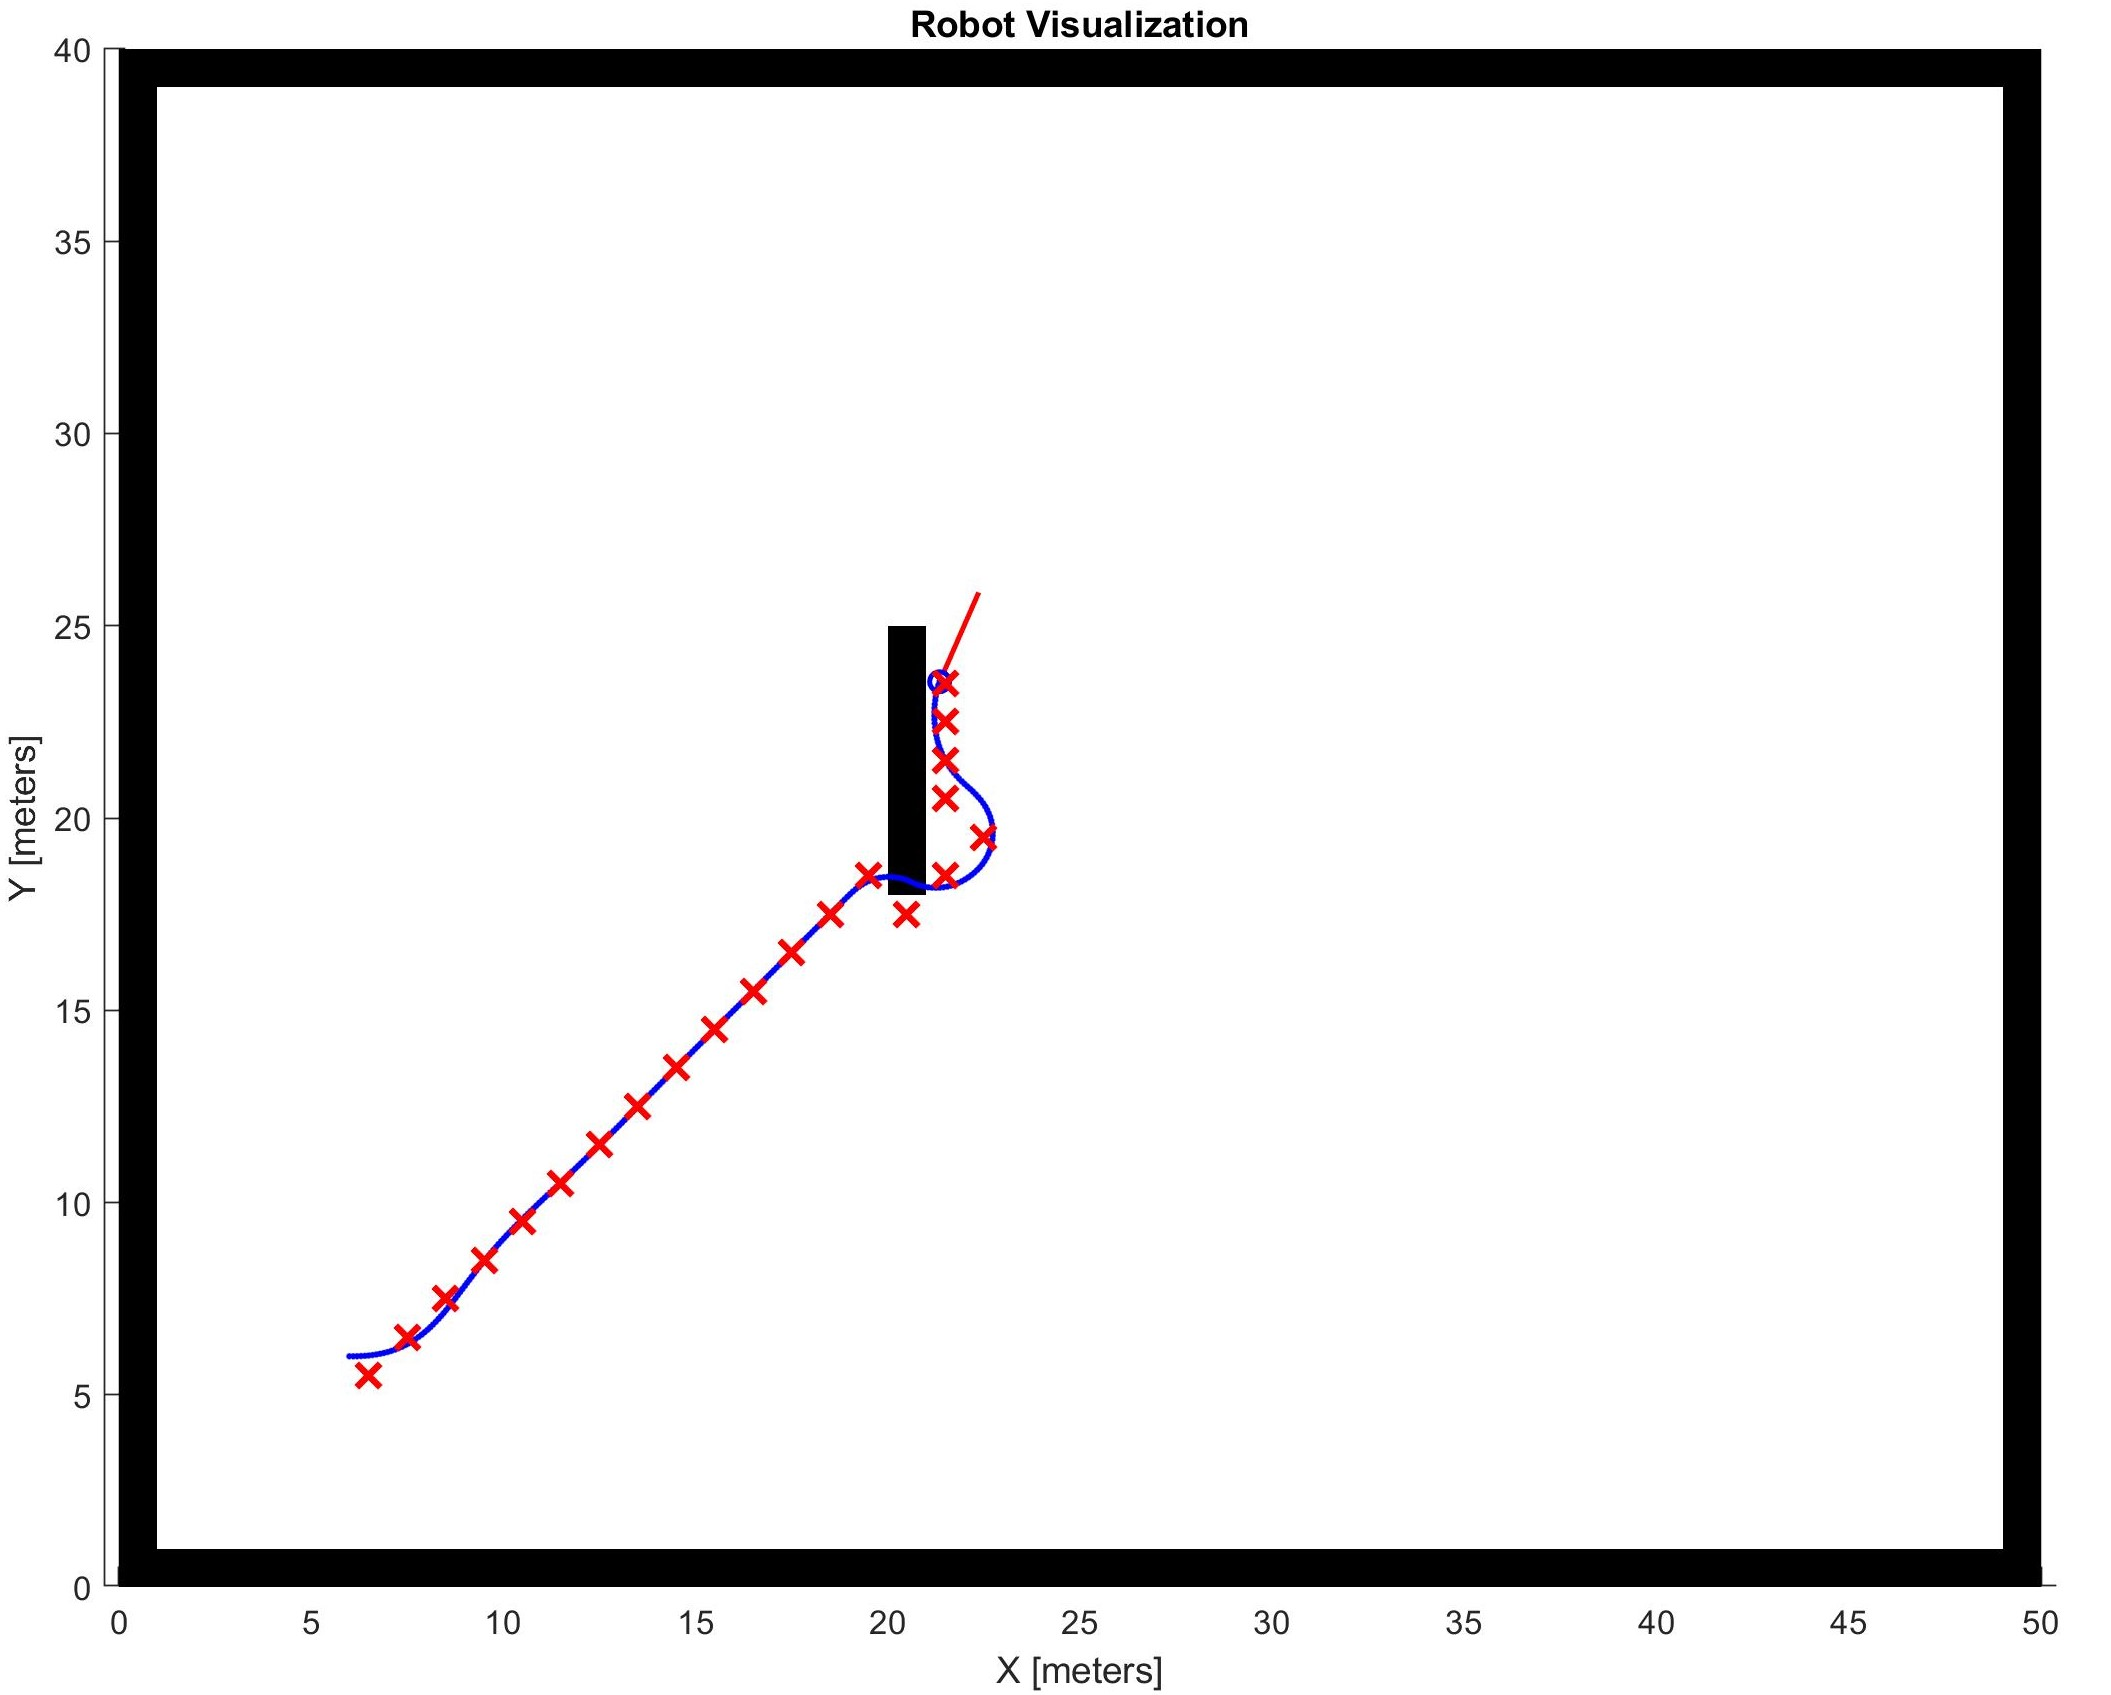
\includegraphics[scale=0.3]{Images/QL path R=-normpos-xy.jpg}
	\caption{نتیجه الگوریتم \lr{Q-learning} برای یادگیری با $R=-\frac{\|(y-goal)\|_2 - \|(x-goal)\|_2}{1000}$}
\end{figure}

در نتیجه این مثال‌ها نشان‌دهنده اهمیت انتخاب صحیح تابع پاداش هستند.














